% FONTE TEMA https://github.com/matze/mtheme
\documentclass[aspectratio=1610]{beamer}
%\documentclass[aspectratio=1610, handout]{beamer}
\usepackage[utf8]{inputenc}
\usepackage{ragged2e}
\usepackage{xcolor}
\usepackage[italian]{babel}
\usepackage{multirow}
\usepackage{silence}
\WarningFilter{beamer}{}
\WarningFilter{metropolis}{}
\usetheme[progressbar=frametitle,titleformat=smallcaps]{metropolis}
\setbeamertemplate{frame numbering}[fraction]
\setbeamercovered{dynamic}
\definecolor{rosso}{RGB}{255, 0, 0}
\definecolor{giallo}{RGB}{254,212,23}
\hypersetup{colorlinks=true,linkcolor=black,urlcolor=rosso}
\setbeamercolor{palette primary}{fg=black, bg=giallo}
\setbeamercolor{background canvas}{bg=white}
\setbeamercolor{normal text}{fg=black}
\setbeamercolor{progress bar}{fg=rosso}
\setbeamercolor{framesubtitle}{fg=rosso}
\setbeamercolor{normal text .dimmed}{fg=giallo}
\setbeamercolor{block title alerted}{fg=rosso, bg=giallo}
\setbeamerfont{caption}{size=\tiny}
\setbeamerfont{caption name}{size=\tiny}
\setlength{\abovecaptionskip}{0pt}
\makeatletter
\metroset{block=fill}
\setlength{\metropolis@progressinheadfoot@linewidth}{1pt} 
\setlength{\metropolis@progressonsectionpage@linewidth}{1pt}
\setlength{\metropolis@titleseparator@linewidth}{1pt}
\makeatother

\title{INTELLIGENZA ARTIFICIALE GENERATIVA}
\subtitle{Cos'è? Come funziona? Problemi?!}
\date{}
\institute{\textit{
        Fonti:
        \begin{itemize}
            \item[-] \href{https://towardsdatascience.com/understanding-llms-from-scratch-using-middle-school-math-e602d27ec876/}{Towards Data Science}
            \item[-] \href{https://www.wired.it/article/intelligenza-artificiale-dati-addestramento-razzismo-sessismo-colonialismo-digitale/}{Grace Browne (Wired)}
            \item[-] \href{https://www.ibm.com/it-it/think/topics/ai-bias}{IBM: Ai Bias}
            \item[-] \href{https://en.wikipedia.org/wiki/AI_slop}{Wikipedia: AI slop}
            \item[-] \textcolor{red}{\href{}{Articoli presenti nelle didascalie delle immagini}} 
        \end{itemize}
    }
}

\begin{document}

\begin{frame}[plain, noframenumbering]
    \titlepage
\end{frame}

\section{MODELLI TRASFORMATIVI}

\begin{frame}{RETI NEURALI}
    \begin{alertblock}{DEFINIZIONE}
        \begin{minipage}{0.98\linewidth}
            \justifying
            Una rete neurale artificiale (\textbf{NN}) è un modello computazionale ispirato alla struttura 
            e al funzionamento del cervello umano. È composta da unità chiamate \textbf{neuroni artificiali} 
            organizzati in strati, che possono prendere in input dei numeri e possono emettere in output altri numeri.\\
            Il \textbf{Deep learning} è un sottoinsieme del \textbf{Machine Learning} (\textbf{ML}) 
            basato su livelli di reti neurali e sta alla base dell'intelligenza artificiale generativa.\\
            \bigskip
            \tiny{\textbf{Curiosità}}\\
            \tiny{\href{https://www.wired.it/article/frank-rosenblatt-perceptron-intelligenza-artificiale/}{il Mark I Perceptron del 1958}}
        \end{minipage}
    \end{alertblock}
\end{frame}

\begin{frame}{RETI NEURALI}
    \begin{alertblock}{ESEMPIO: CLASSIFICARE UN OGGETTO}
        \begin{minipage}{0.96\linewidth}
            \justifying
            \bigskip
            \textbf{DATI OGGETTO DISPONIBILI}:
            \begin{itemize}
                \item Colore dominante (RGB);
                \item Volume in millilitri.
            \end{itemize}
            Esempio: Dati di una foglia e di un girasole:\\
            \begin{center}
                \begin{tabular}{c c c}
                    & \textbf{Foglia} & \textbf{Fiore} \\
                    \hline
                    \hline
                    \textbf{R} & 32 & 241 \\
                    \hline
                    \textbf{G} & 107 & 200 \\
                    \hline
                    \textbf{B} & 56 & 4 \\
                    \hline
                    \textbf{Vol} & 11.2 & 59.5 \\
                \end{tabular}
            \end{center}
        \end{minipage}
    \end{alertblock}
\end{frame}

\begin{frame}{ESEMPIO: CLASSIFICARE UN OGGETTO (FOGLIA O FIORE?)}
    \only<1 | handout:0>{\begin{figure}
        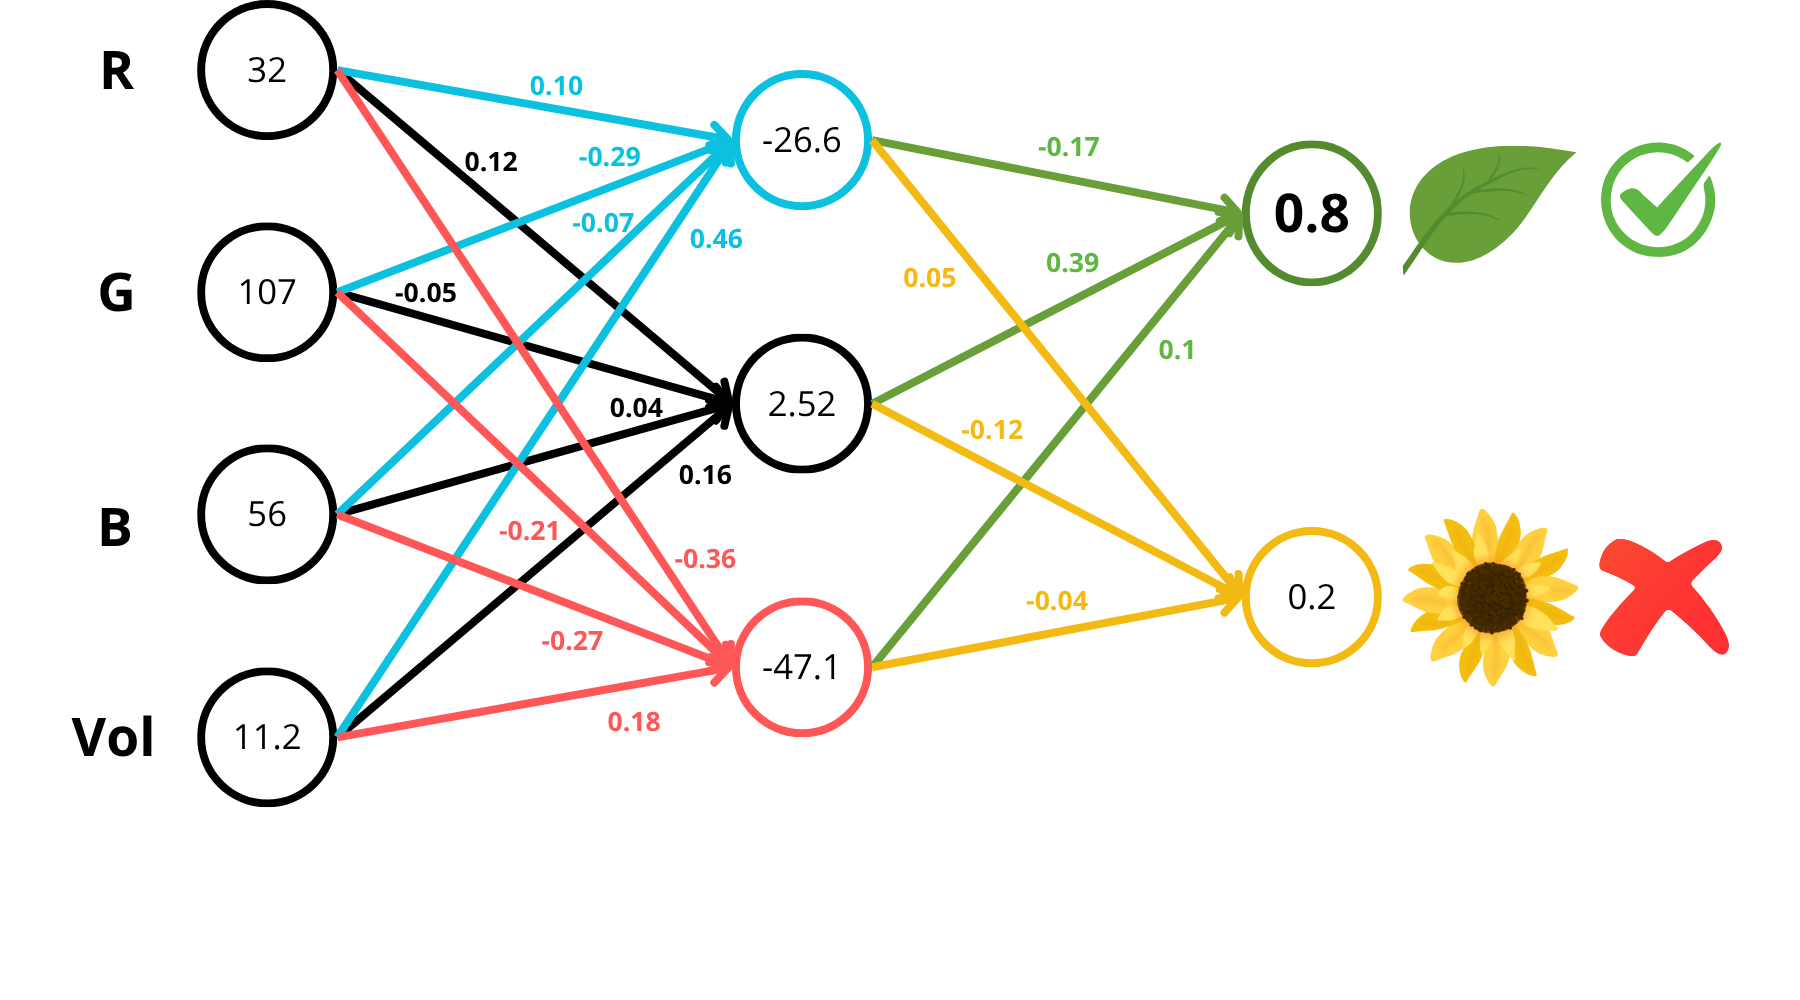
\includegraphics[width=\linewidth]{img/reteNeurale1.png}
        \caption{{creata con \href{www.canva.com}{Canva}}}
    \end{figure}}
    \only<2 | handout:1>{\begin{figure}
        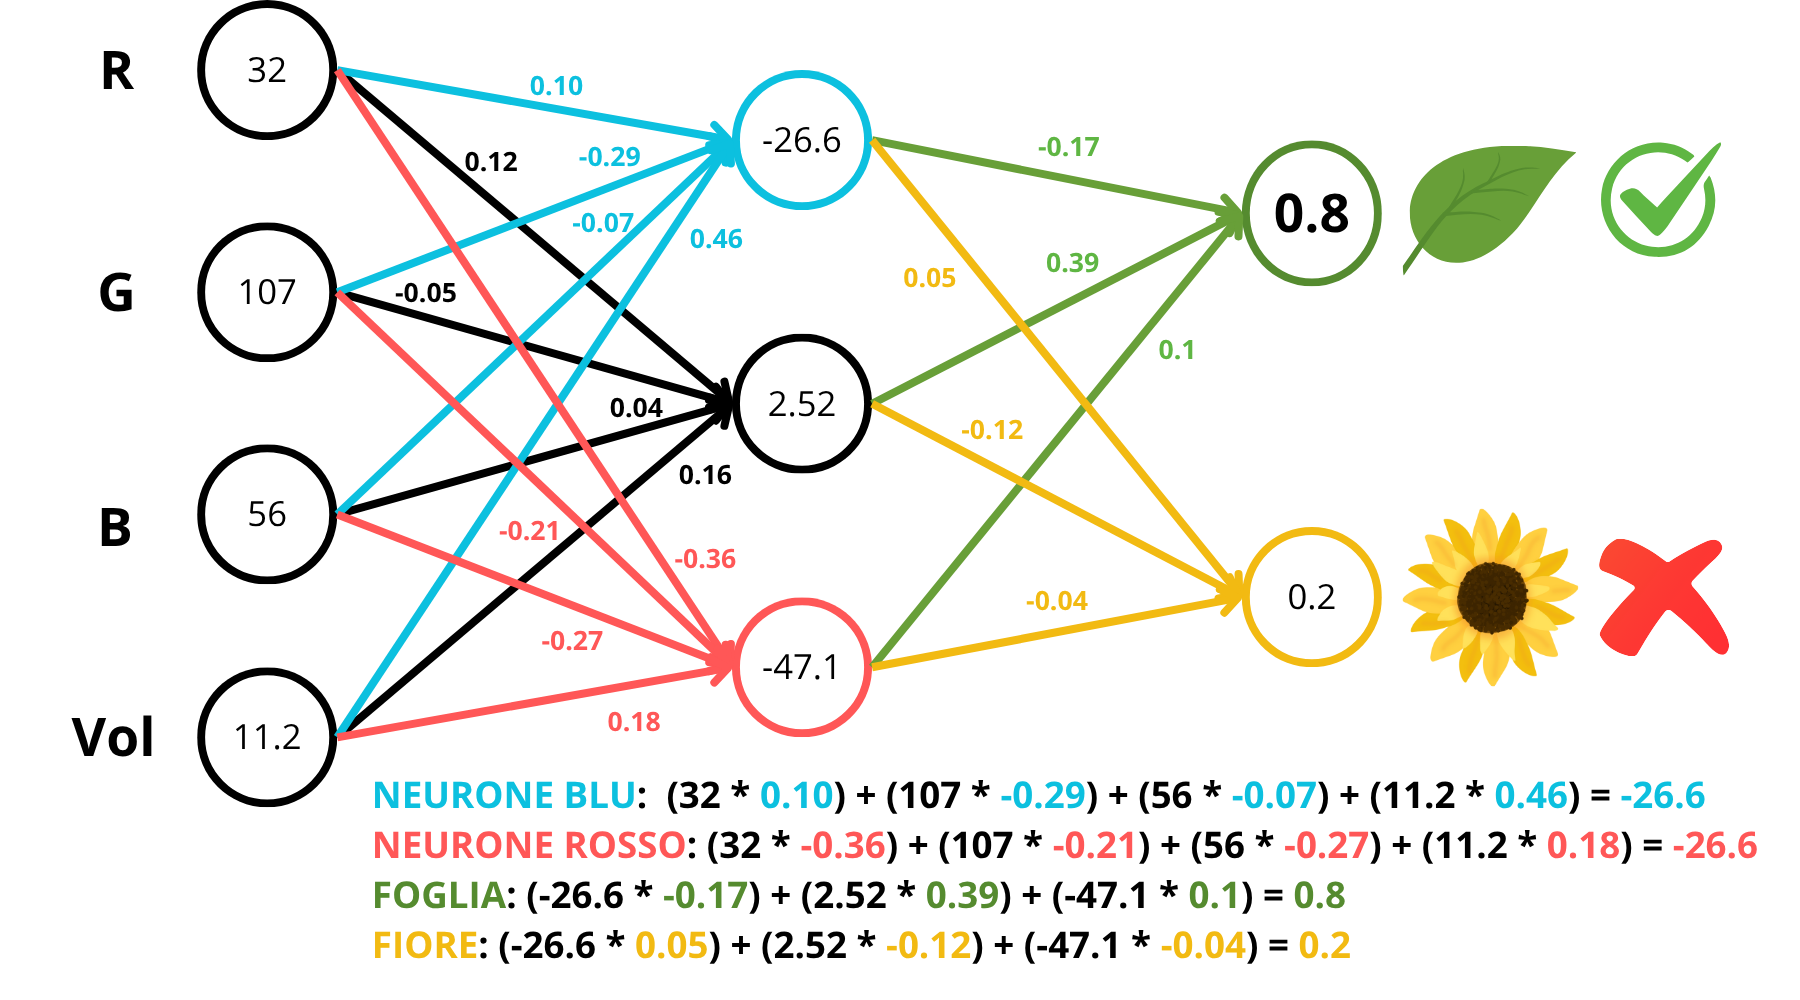
\includegraphics[width=\linewidth]{img/reteNeurale2.png}
        \caption{{creata con \href{www.canva.com}{Canva}}}
    \end{figure}}
\end{frame}

\section{DEFINIZIONI}

\begin{frame}{ELEMENTI DI UNA RETE NEURALE}
    \only<1 | handout:0>{\begin{figure}
        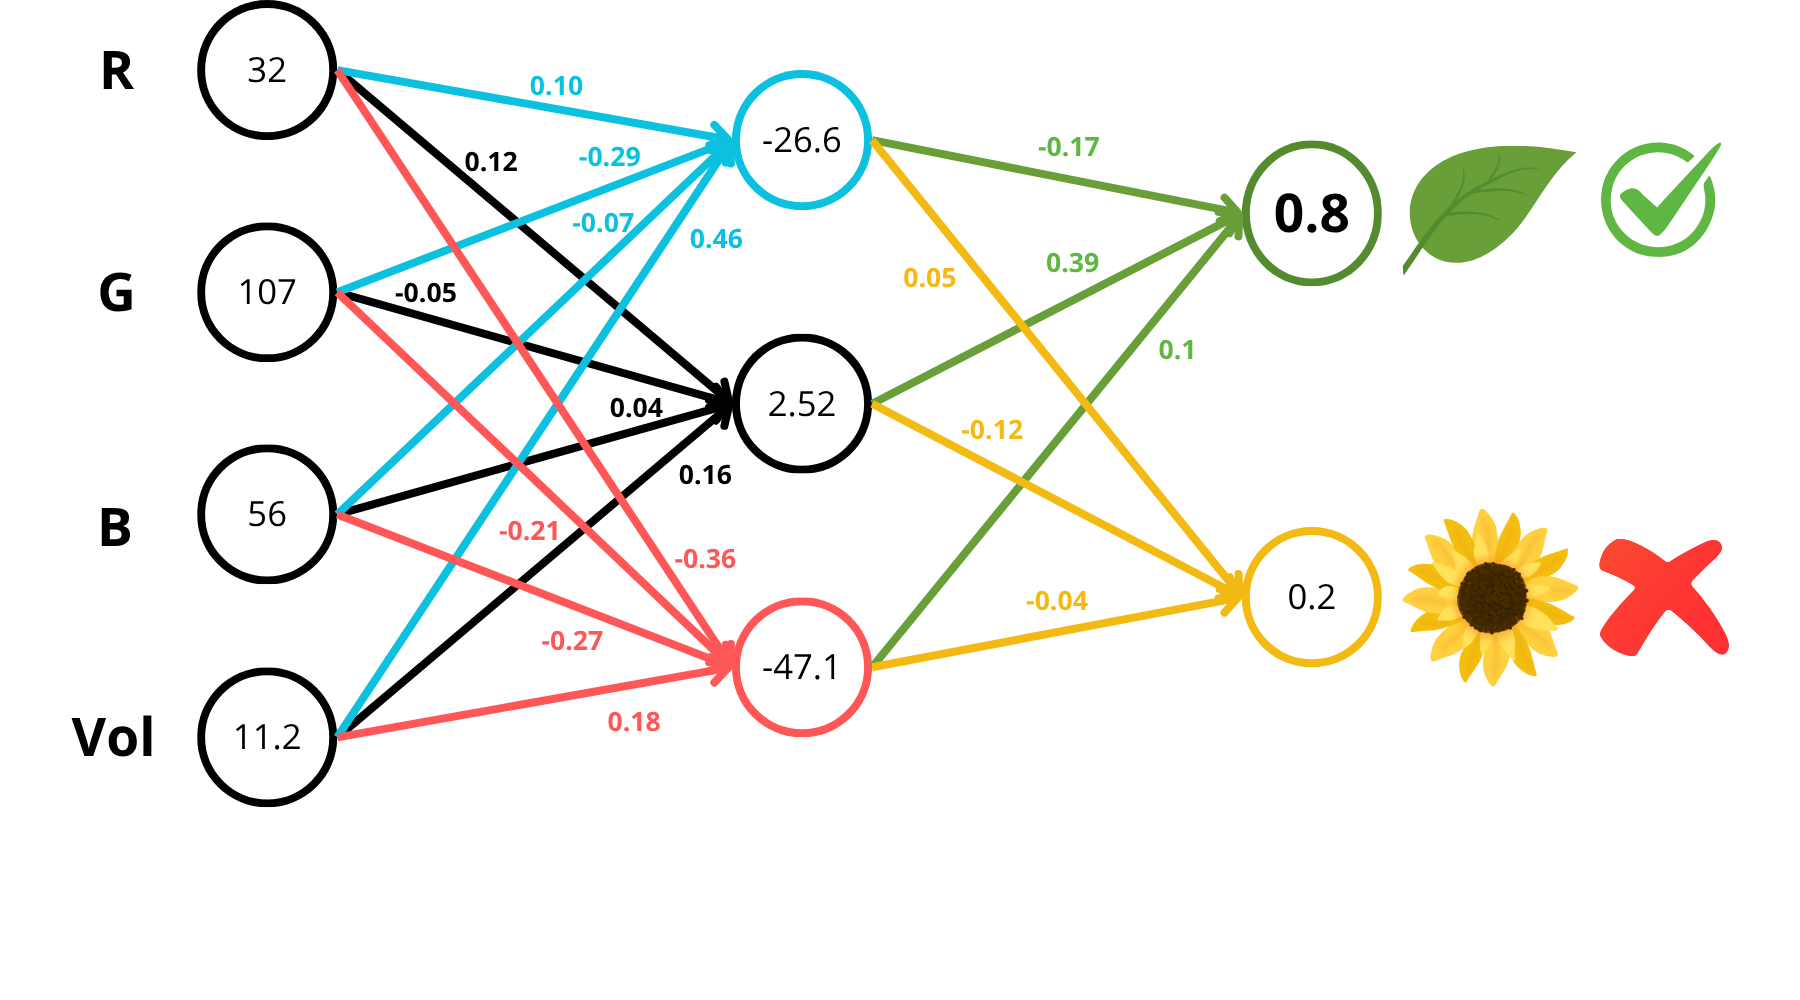
\includegraphics[width=\linewidth]{img/reteNeurale1.png}
        \caption{{creata con \href{www.canva.com}{Canva}}}
    \end{figure}}
    \only<2 | handout:1>{\begin{figure}
        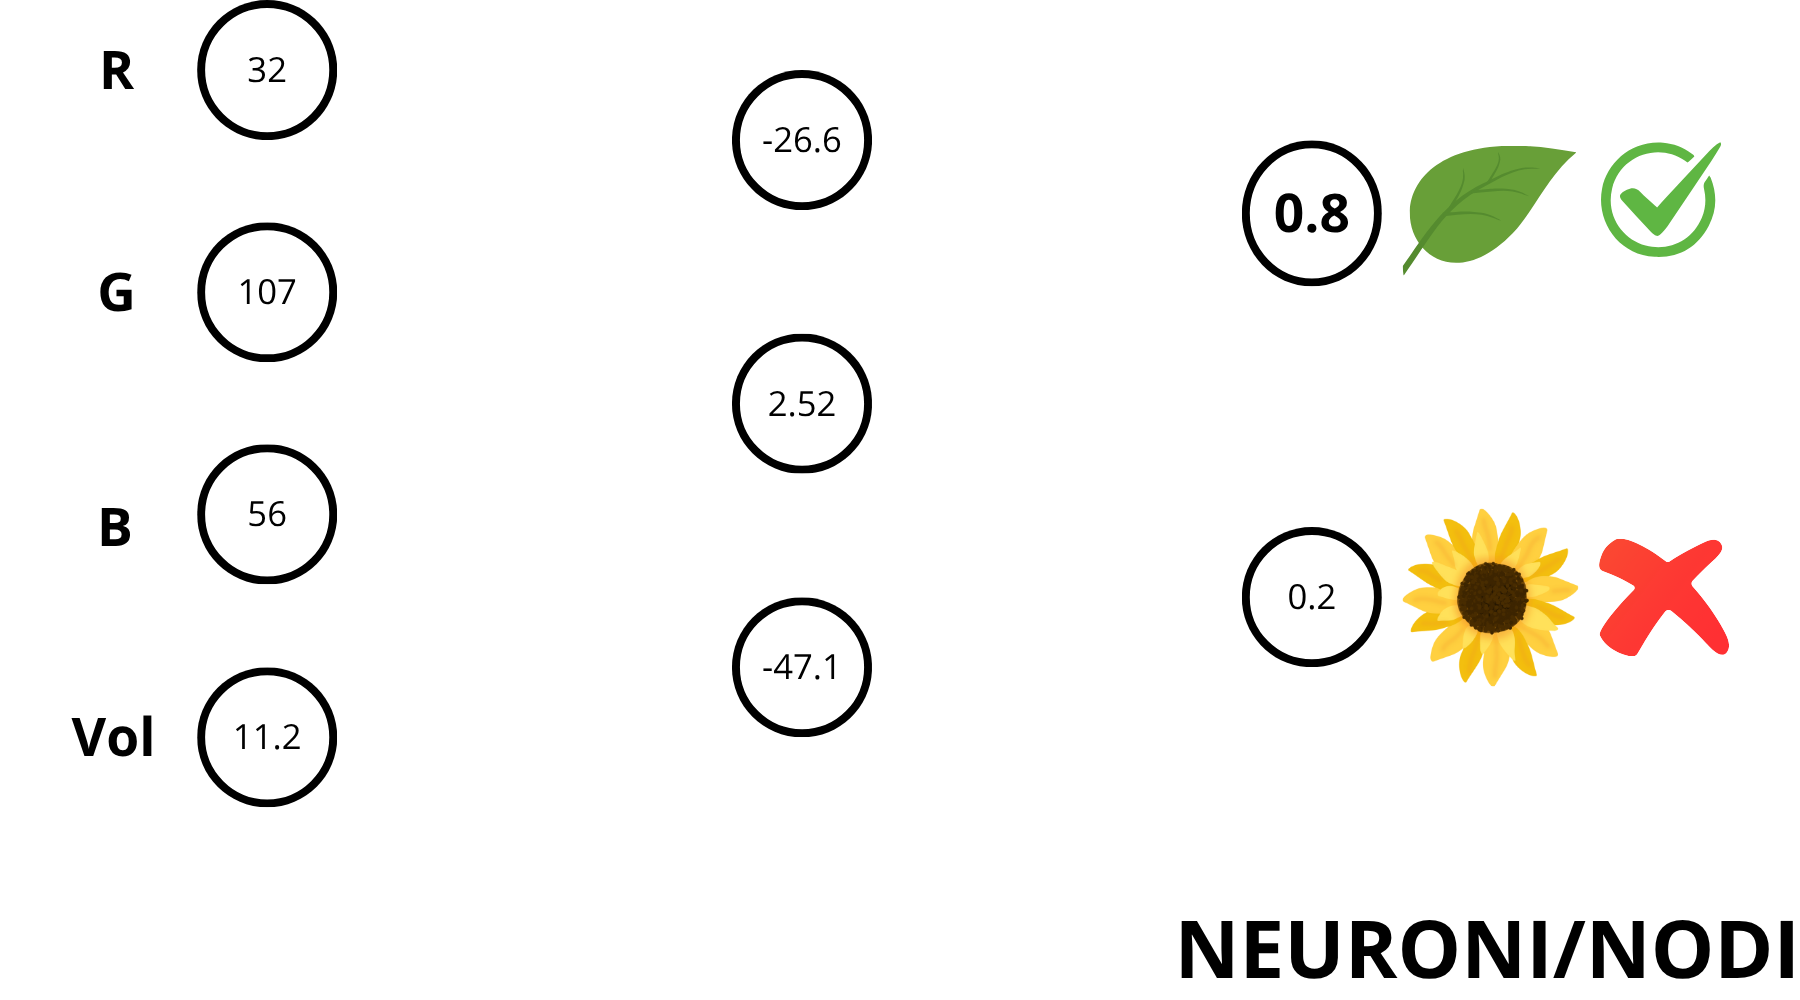
\includegraphics[width=\linewidth]{img/reteNeurale3.png}
        \caption{{creata con \href{www.canva.com}{Canva}}}
    \end{figure}}
    \only<3 | handout:0>{\begin{figure}
        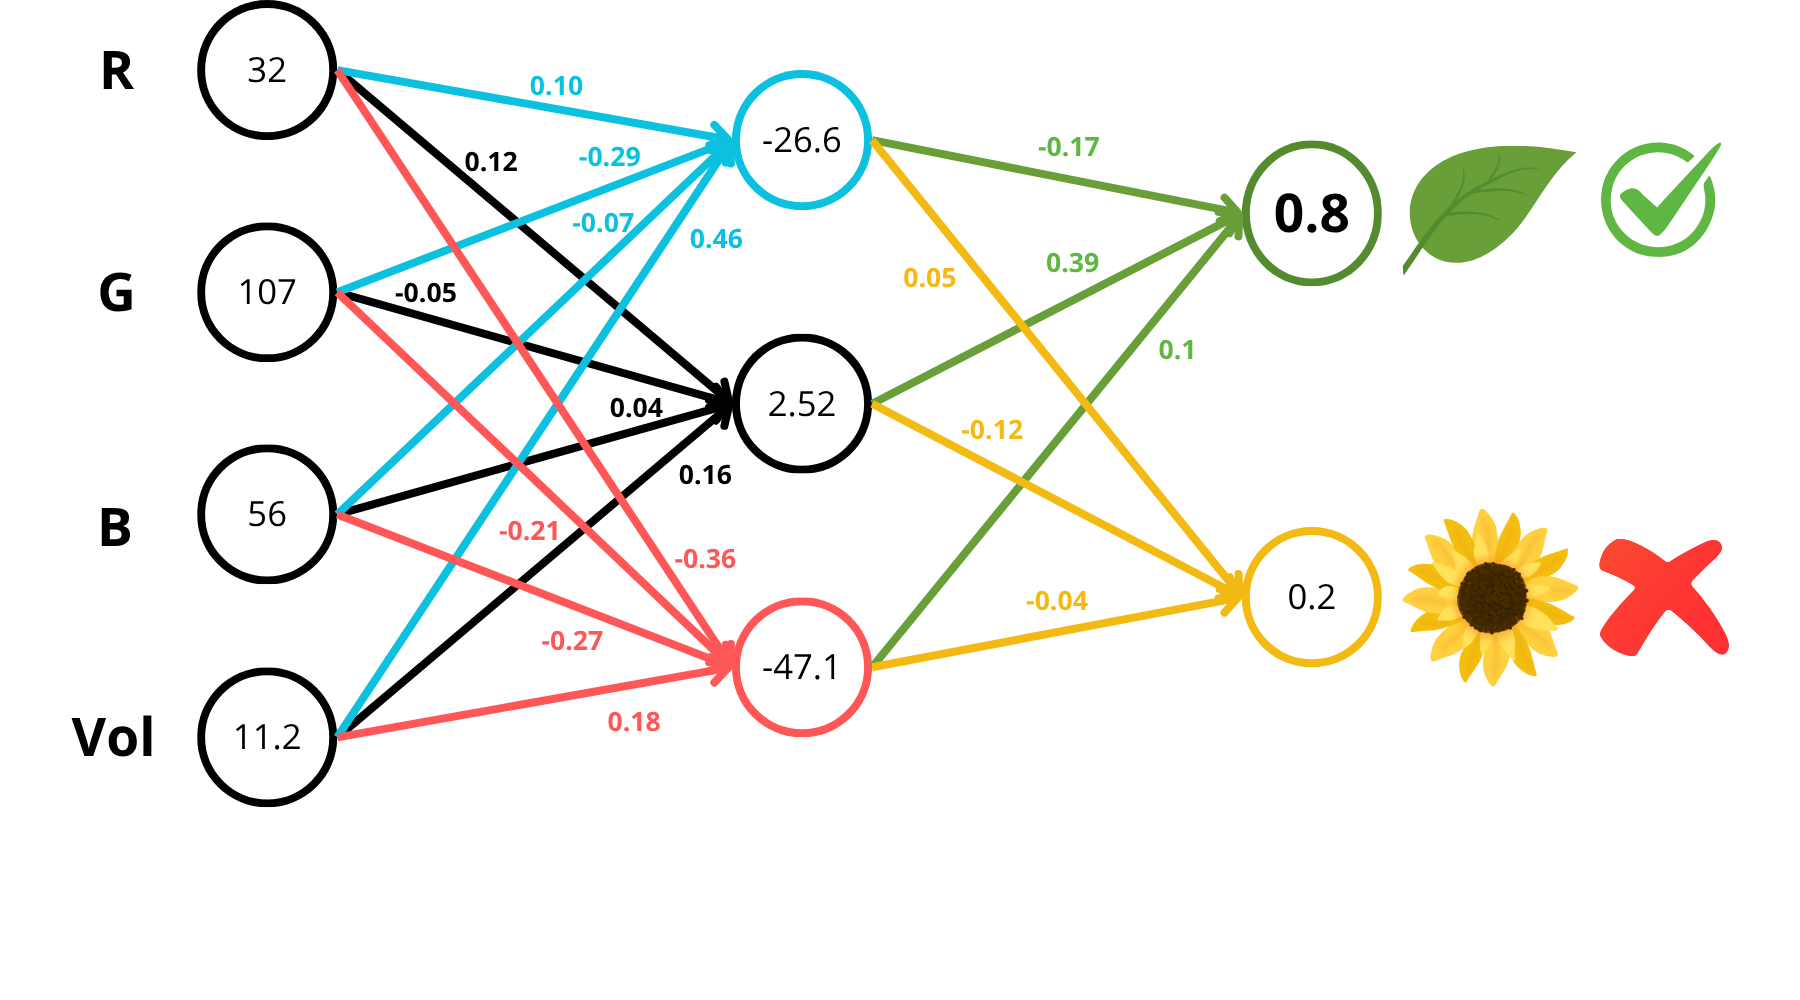
\includegraphics[width=\linewidth]{img/reteNeurale1.png}
        \caption{{creata con \href{www.canva.com}{Canva}}}
    \end{figure}}
    \only<4 | handout:2>{\begin{figure}
        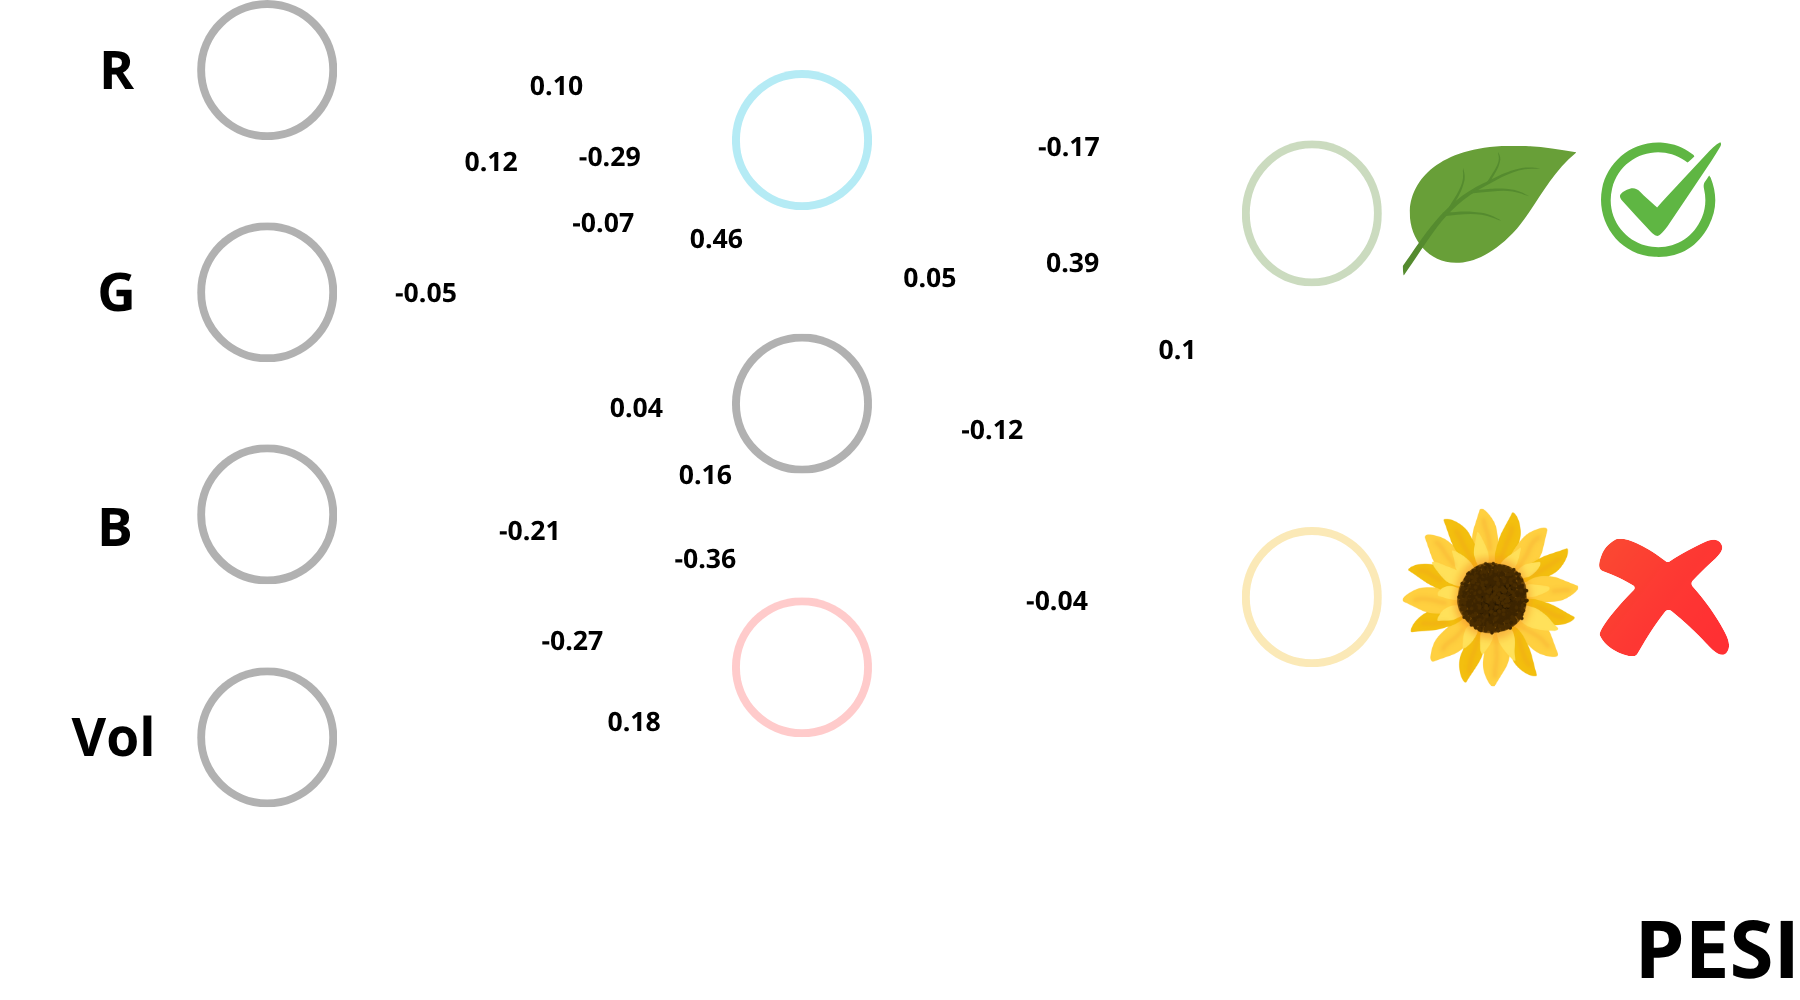
\includegraphics[width=\linewidth]{img/reteNeurale4.png}
        \caption{{creata con \href{www.canva.com}{Canva}}}
    \end{figure}}
    \only<5 | handout:0>{\begin{figure}
        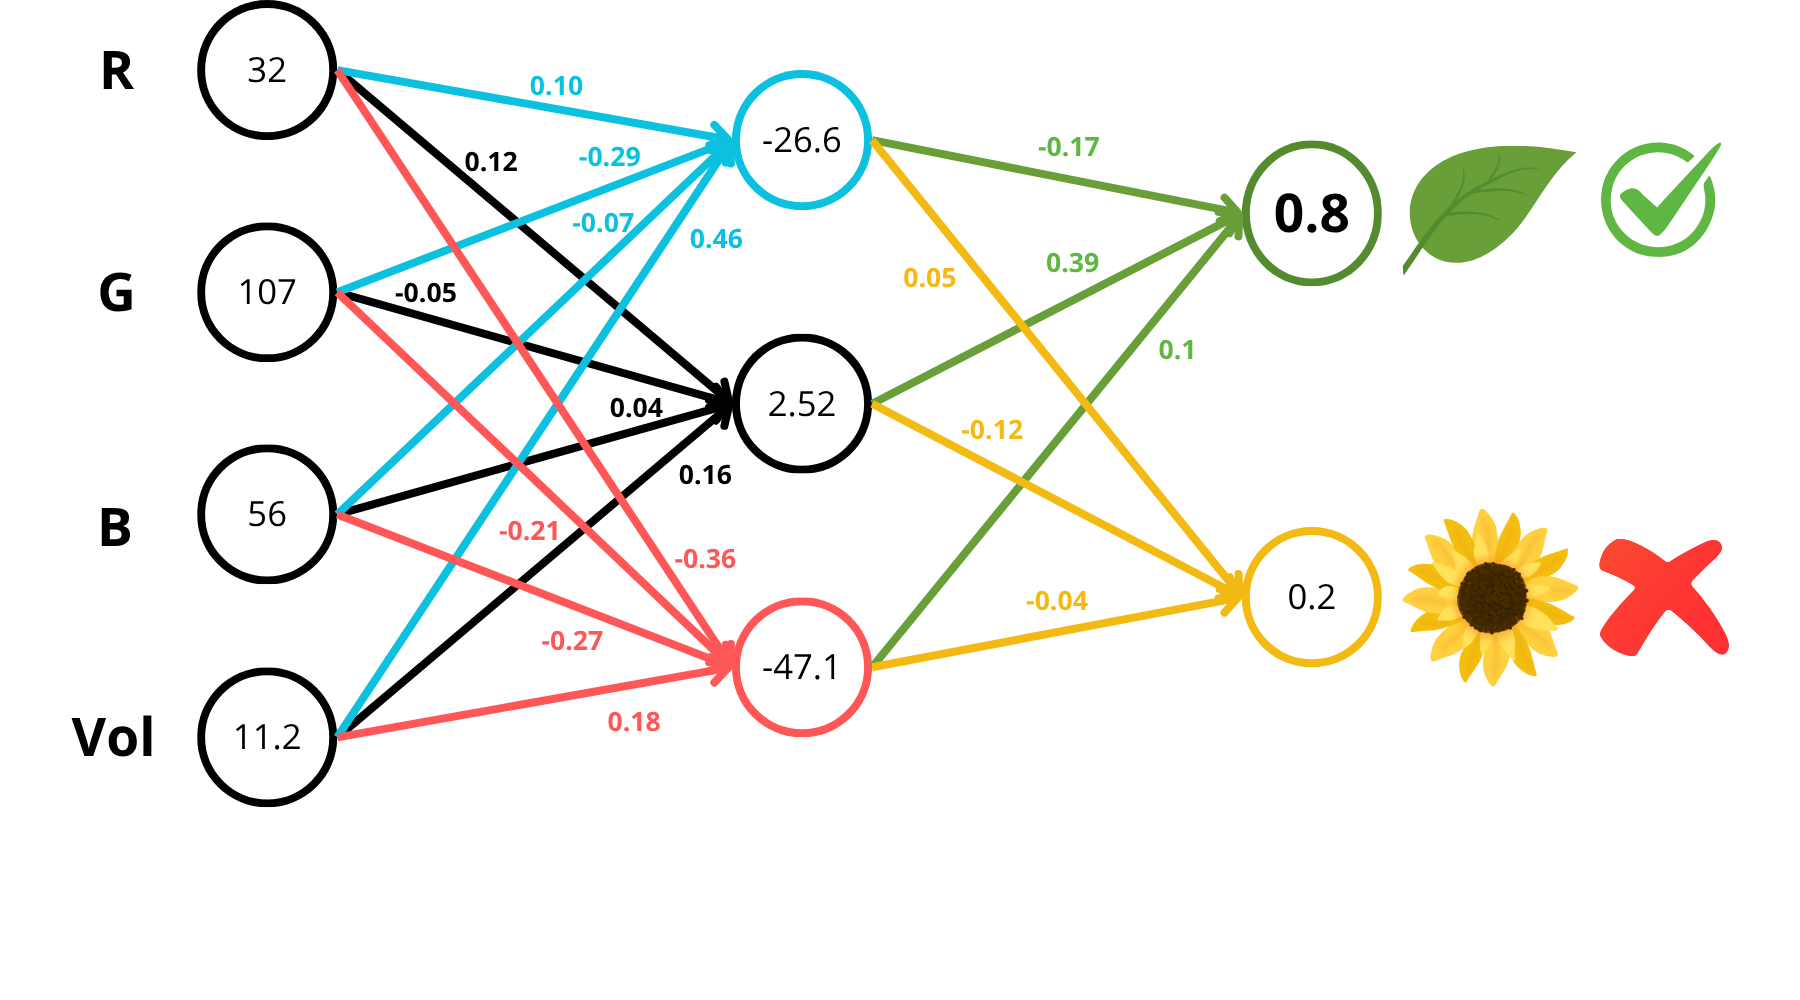
\includegraphics[width=\linewidth]{img/reteNeurale1.png}
        \caption{{creata con \href{www.canva.com}{Canva}}}
    \end{figure}}
    \only<6 | handout:3>{\begin{figure}
        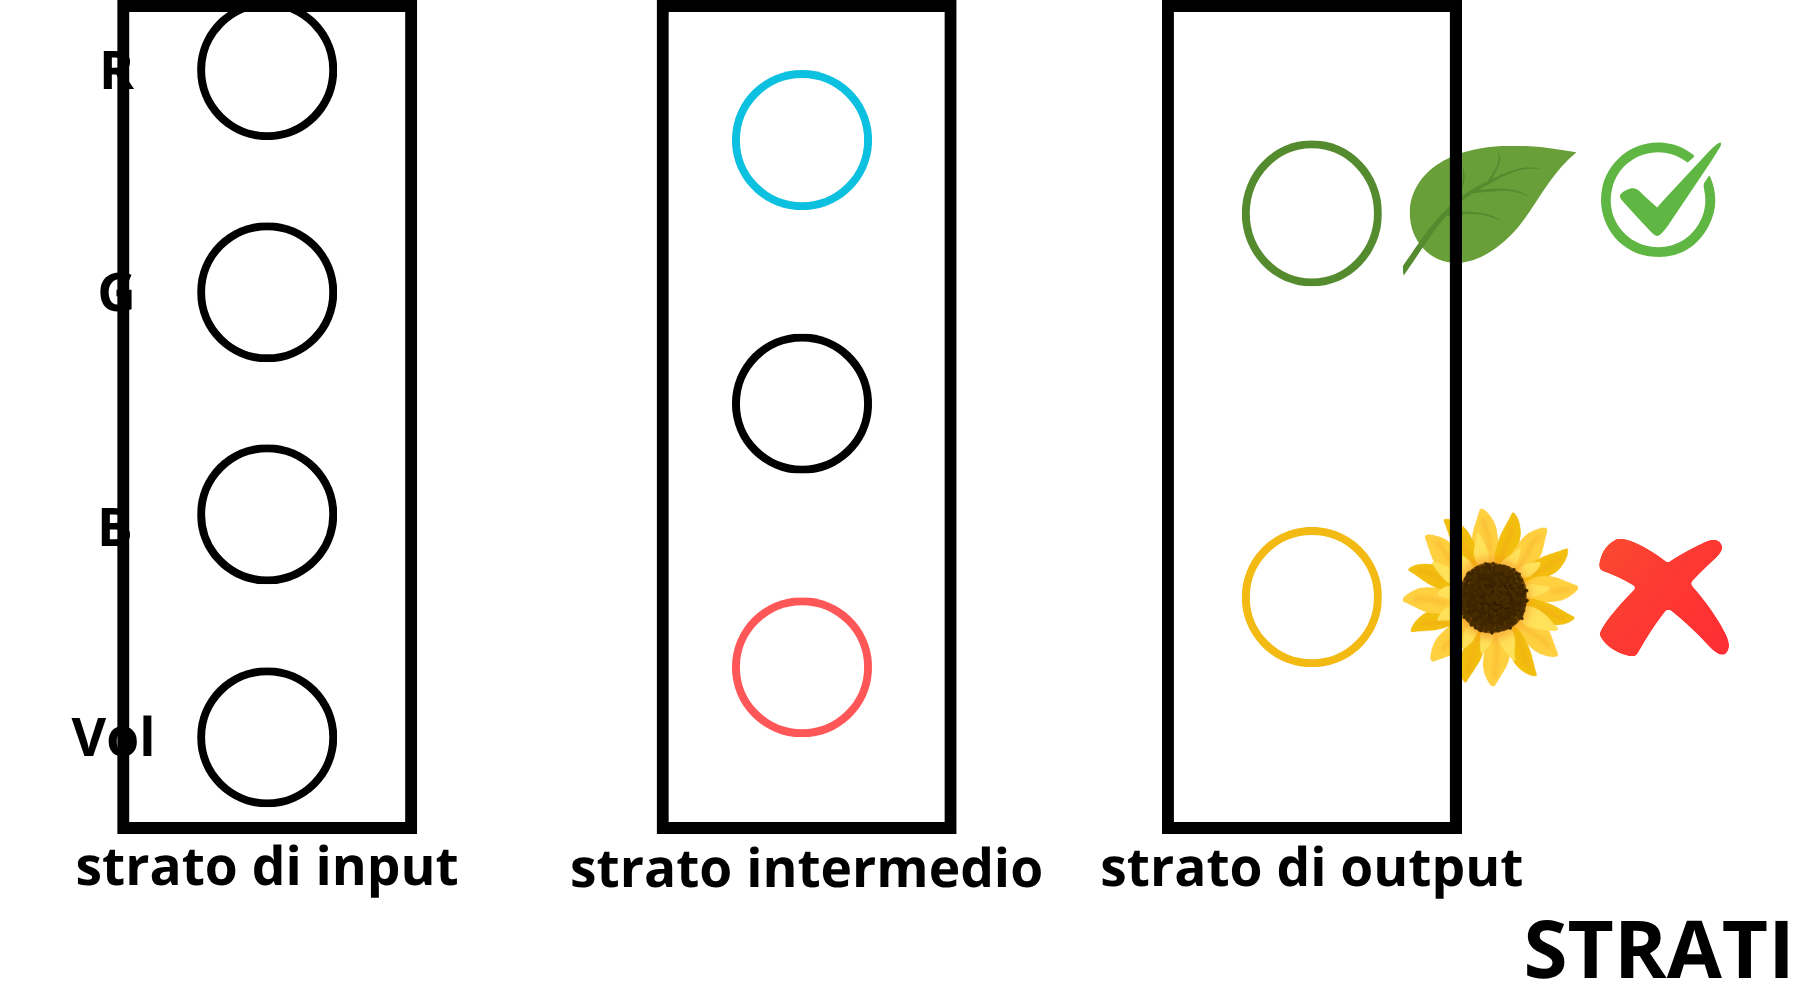
\includegraphics[width=\linewidth]{img/reteNeurale5.png}
        \caption{{creata con \href{www.canva.com}{Canva}}}
    \end{figure}}
\end{frame}

\begin{frame}{ESEMPIO: CLASSIFICARE UN OGGETTO (FOGLIA O FIORE?)}
    \begin{alertblock}{INTELLIGENZA?!}
        \begin{minipage}{0.98\linewidth}
            \justifying
            Il modello \textbf{non ha idea} di cosa sia una foglia o un fiore, 
            o cosa siano (RGB, Vol). Il modello ha semplicemente il compito di prendere esattamente 4 
            numeri e restituire esattamente 2 numeri.\\
            \bigskip
            \textbf{L'INTERPRETAZIONE DEI DATI IN INPUT E OUTPUT SPETTA A NOI}.
        \end{minipage}
    \end{alertblock}
\end{frame}

\section{COME SI DETERMINANO I PESI? \\ ADDESTRARE IL MODELLO}

\begin{frame}{COME SI DETERMINANO I PESI?}
    \begin{alertblock}{TRAINING DATA}
        \begin{minipage}{0.98\linewidth}
            \justifying
            Per poter addestrare il modello e quindi determinare i pesi associati alle connessioni tra i neuroni, 
            è necessario fornire al modello un insieme di dati di addestramento (\textbf{training data}), i quali 
            contengono esempi di input e i corrispondenti output desiderati.\\
            I dati vengono quindi \textbf{etichettati} in modo che il modello possa apprendere la relazione 
            tra input e output.\\
            Nell'esempio precedente i dati di addestramento etichettati potrebbero essere: 
            \begin{itemize}
                \item Input: [32, 107, 56, 11.2] $\rightarrow$ Output desiderato: foglia;
                \item Input: [241, 200, 4, 59.5] $\rightarrow$ Output desiderato: fiore.
            \end{itemize}
        \end{minipage}
    \end{alertblock}
\end{frame}

\begin{frame}{ALGORITMO DI APPRENDIMENTO}
    \only<1 | handout:1>{\begin{figure}
        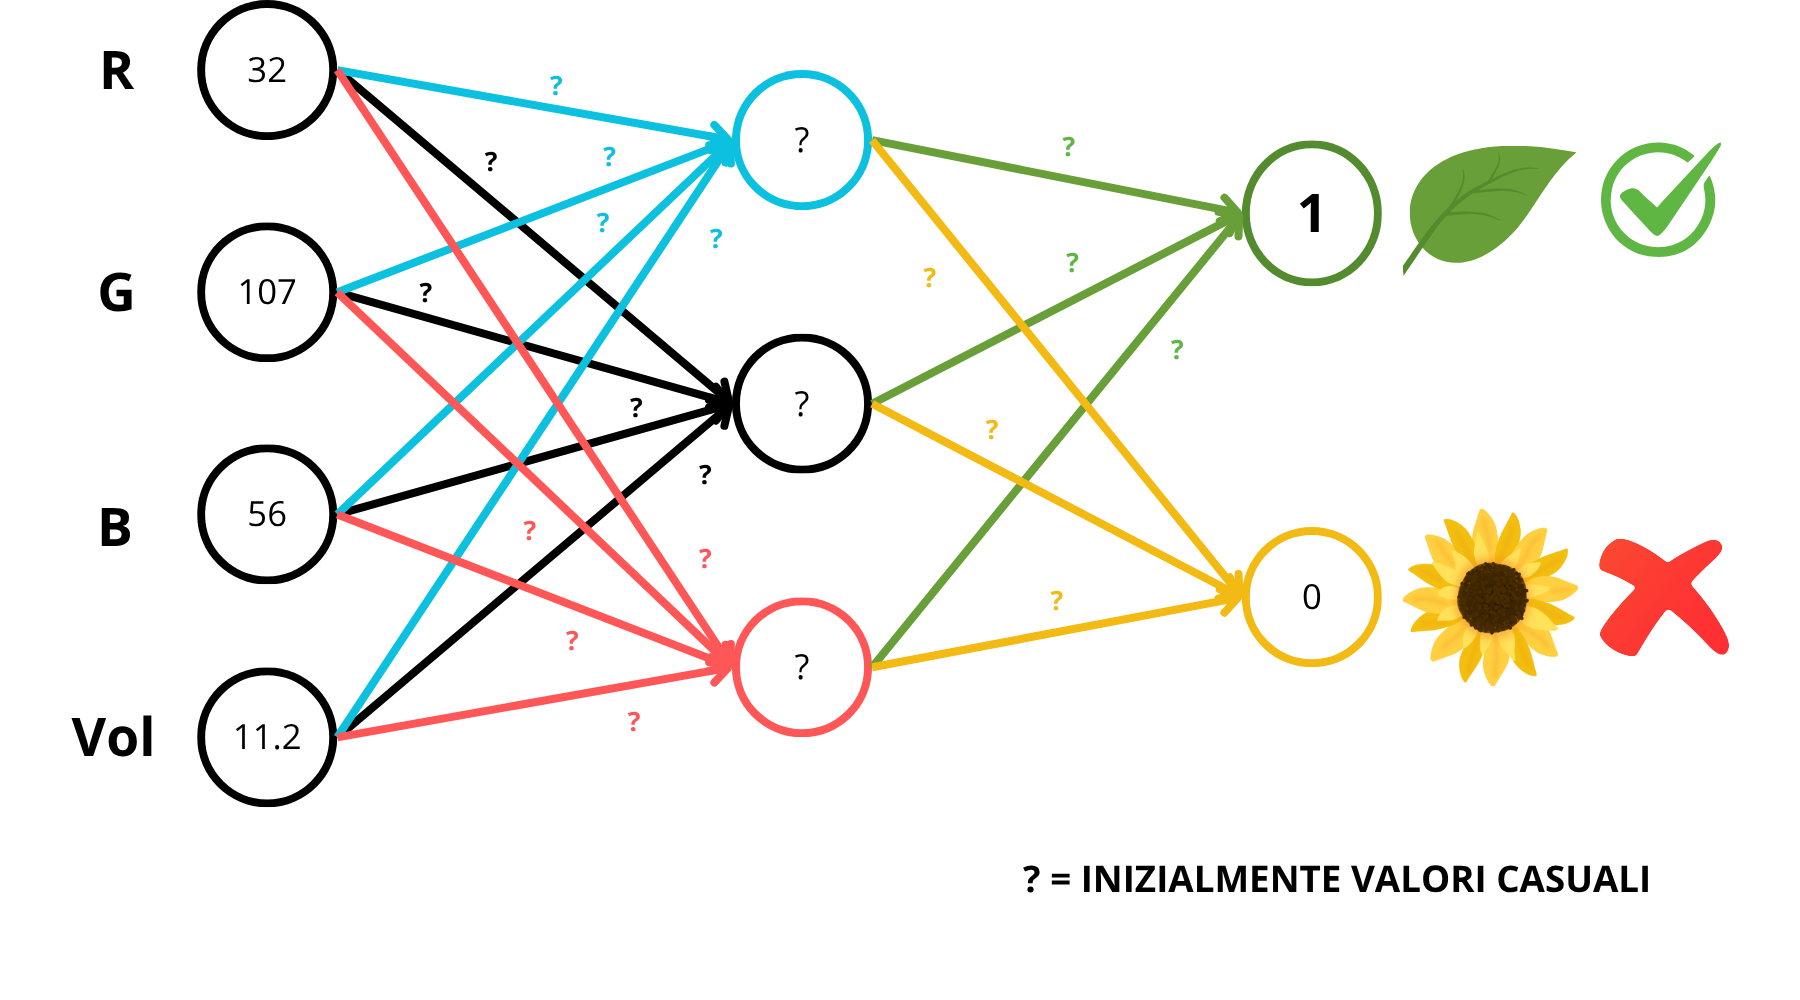
\includegraphics[width=\linewidth]{img/reteNeurale7.png}
        \caption{{creata con \href{www.canva.com}{Canva}}}
    \end{figure}}
    \only<2 | handout:2>{\begin{figure}
        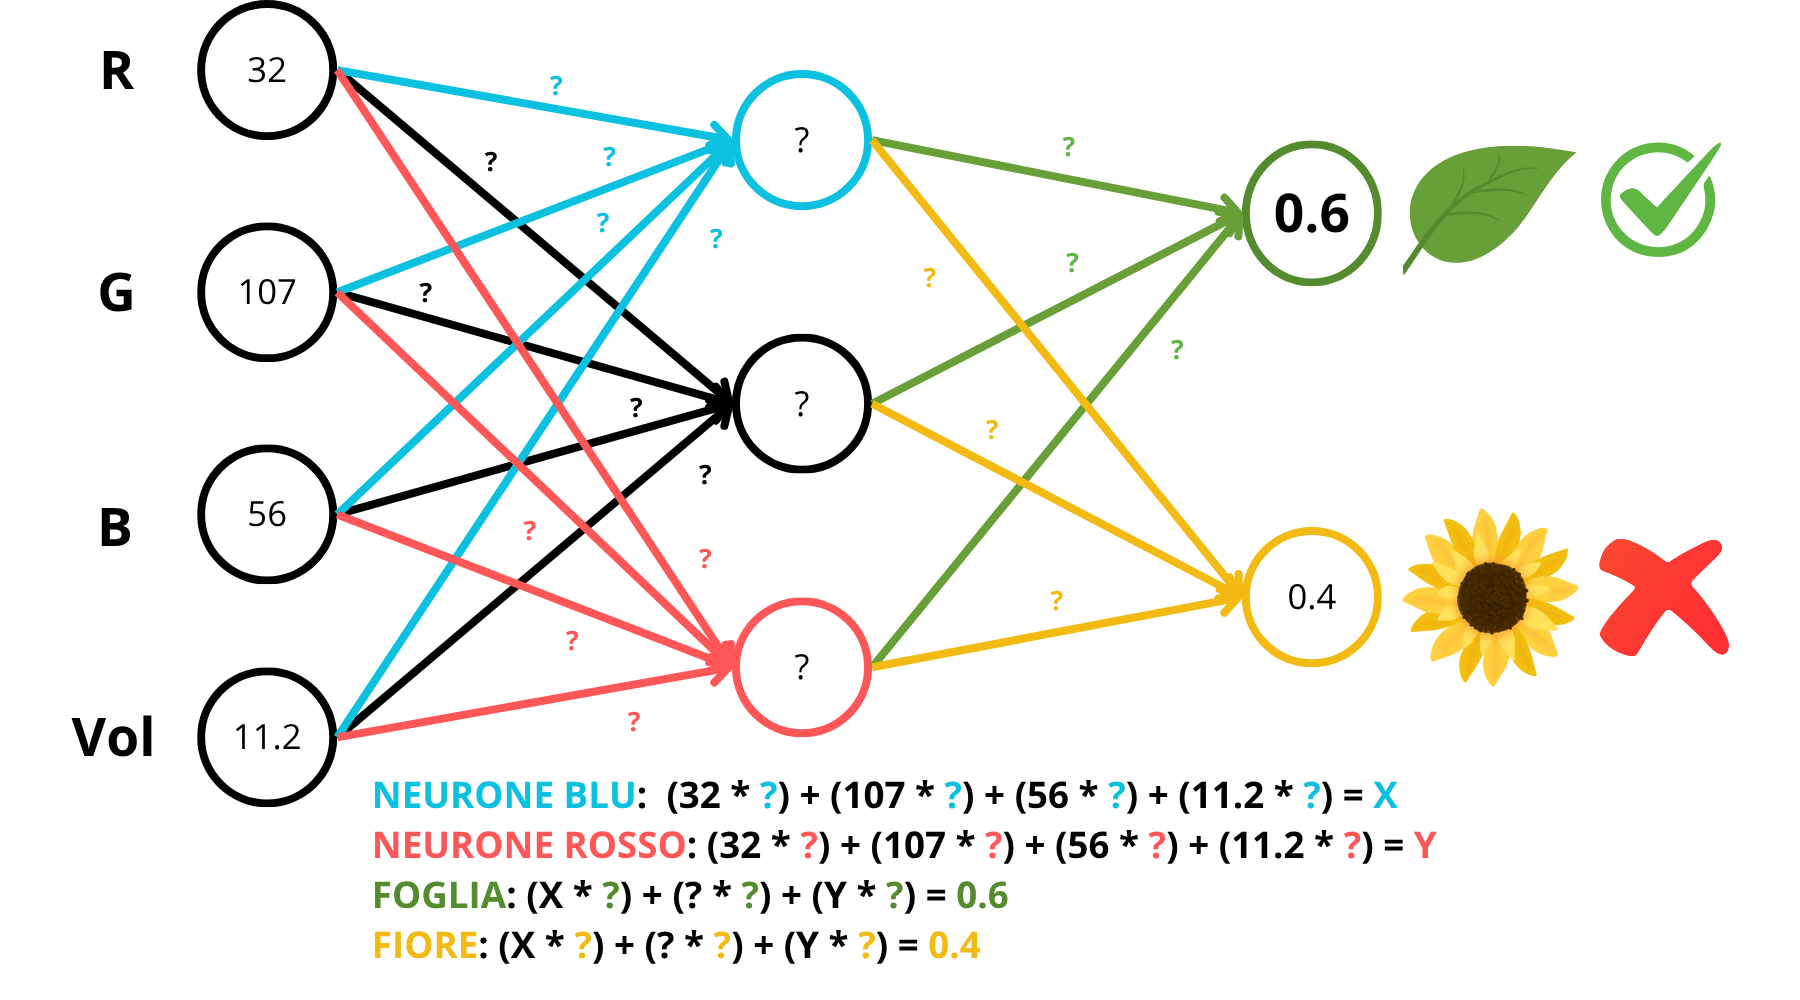
\includegraphics[width=\linewidth]{img/reteNeurale8.png}
        \caption{{creata con \href{www.canva.com}{Canva}}}
    \end{figure}}
    \only<3 | handout:3>{\begin{figure}
        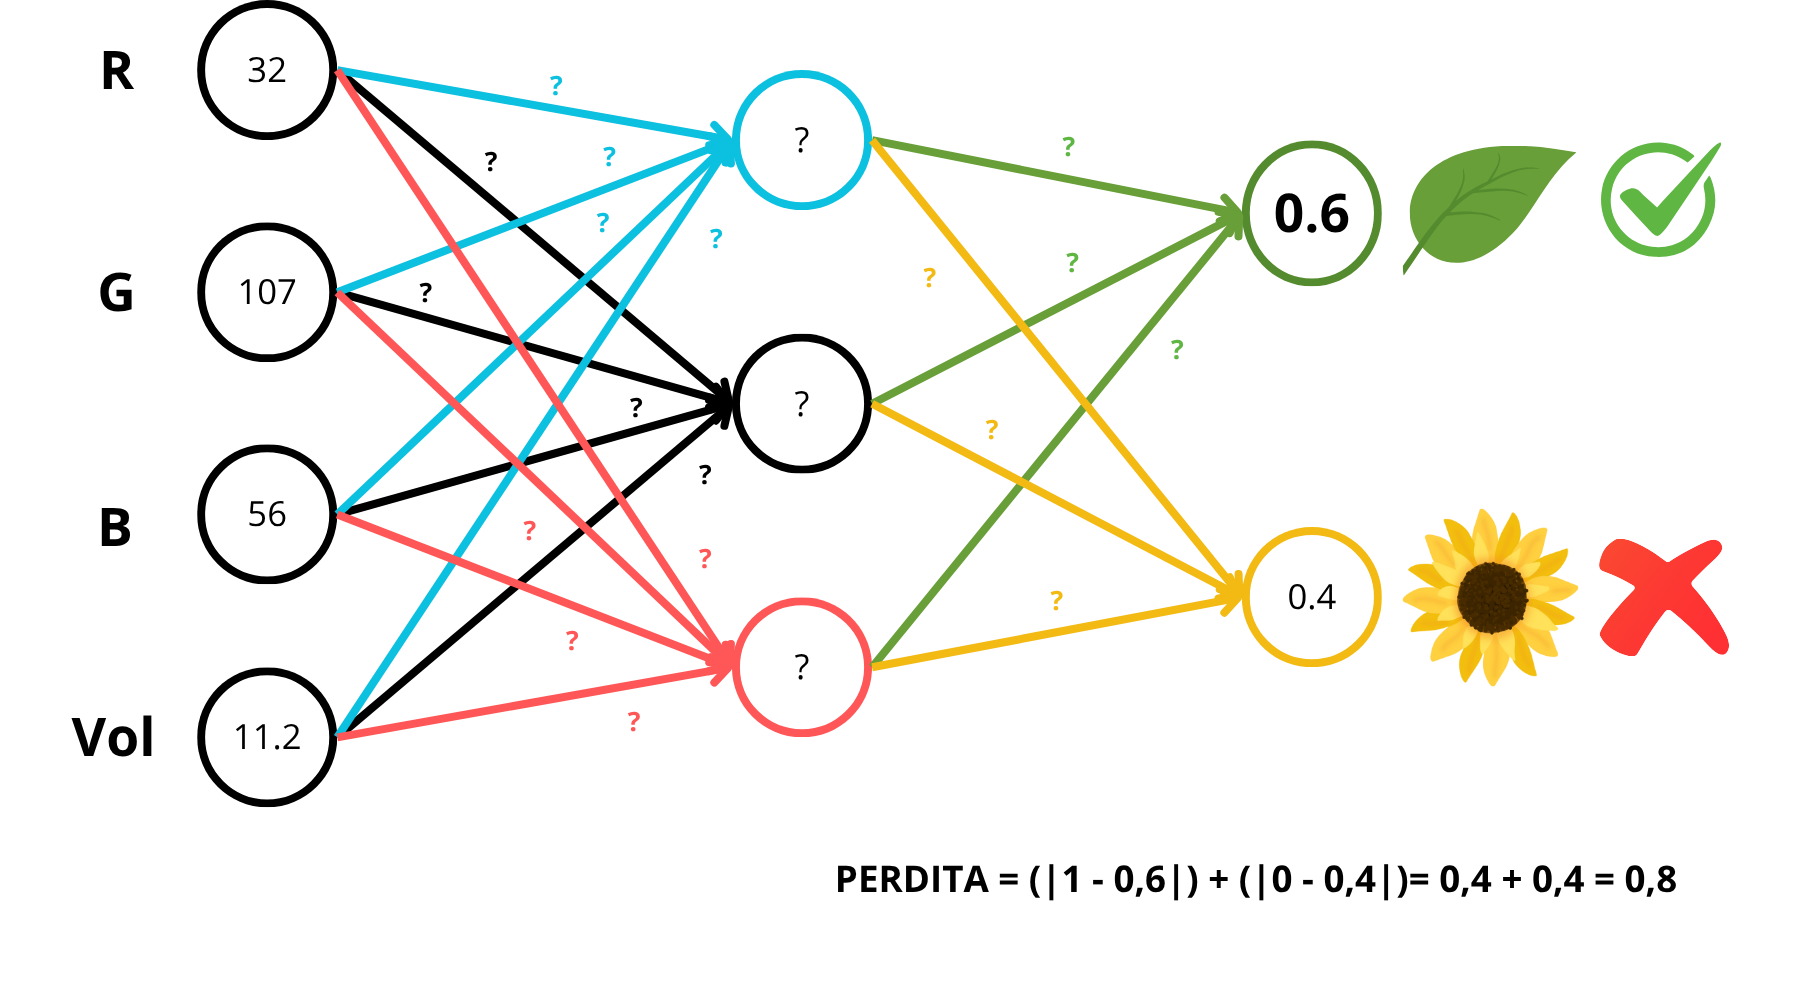
\includegraphics[width=\linewidth]{img/reteNeurale9.png}
        \caption{{creata con \href{www.canva.com}{Canva}}}
    \end{figure}}
    \only<4 | handout:4>{\begin{figure}
        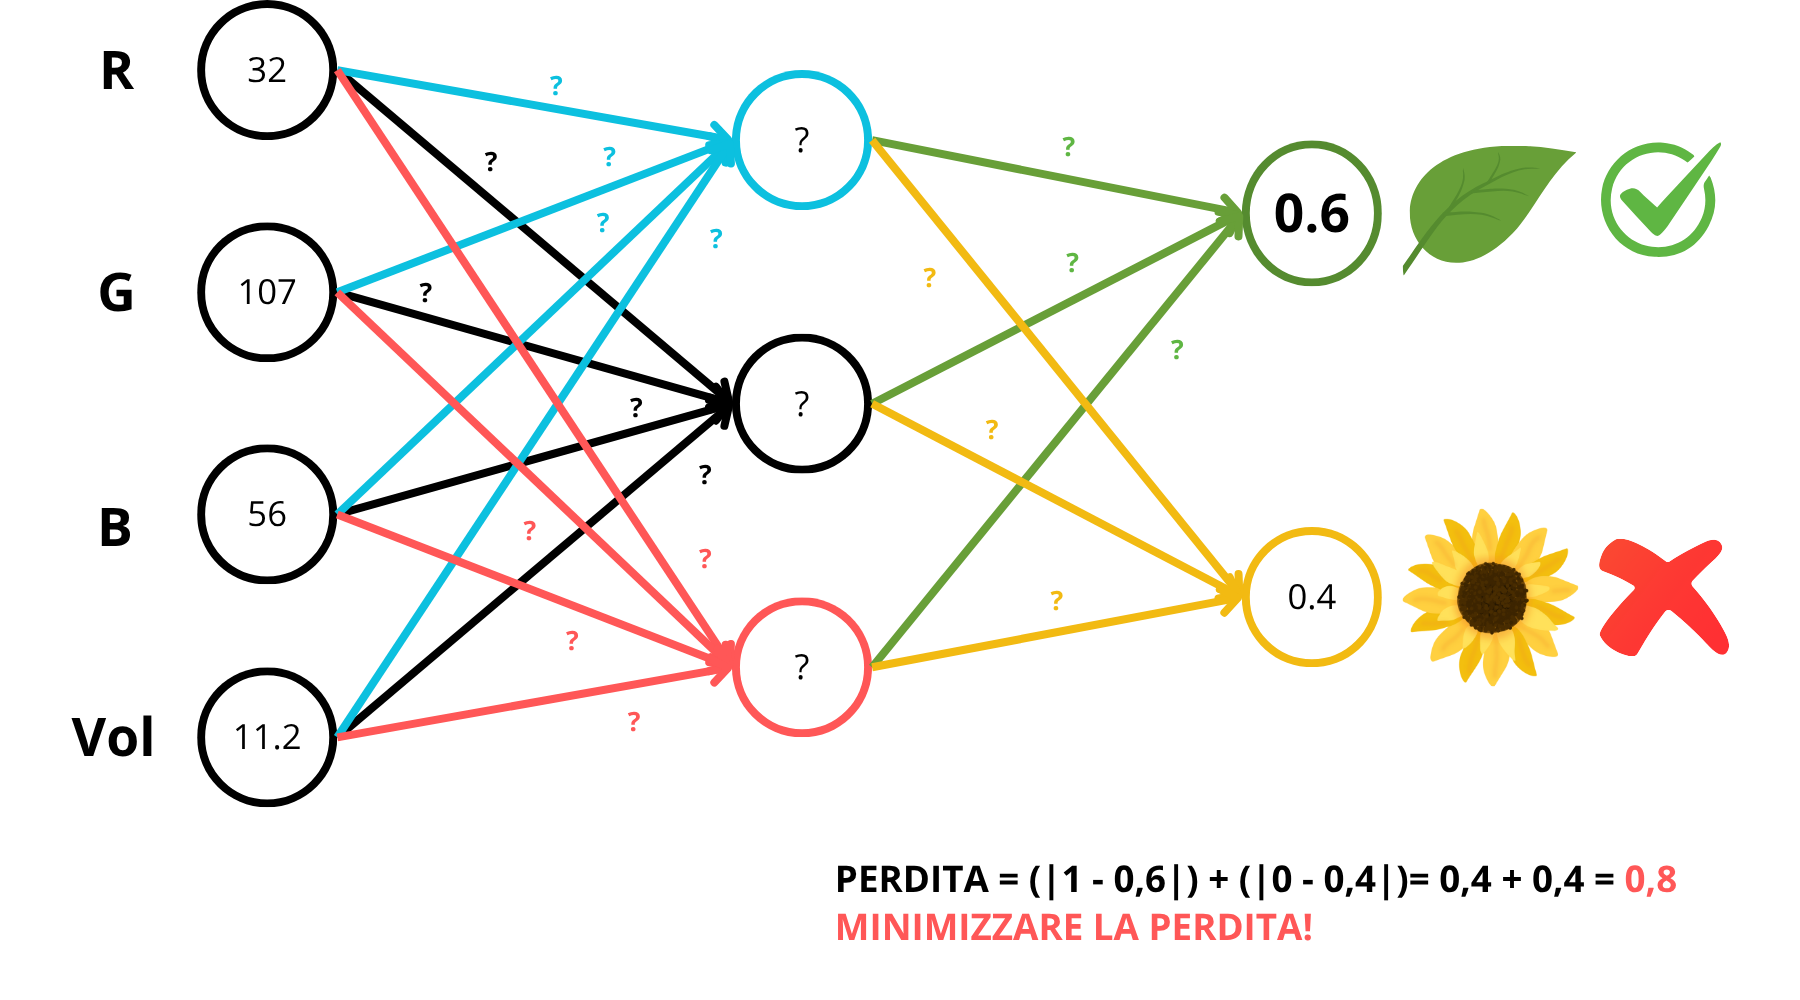
\includegraphics[width=\linewidth]{img/reteNeurale10.png}
        \caption{{creata con \href{www.canva.com}{Canva}}}
    \end{figure}}
\end{frame}

\begin{frame}{ALGORITMO DI APPRENDIMENTO}
    \begin{alertblock}{ALLENAMENTO DEL MODELLO}
        \begin{minipage}{0.98\linewidth}
            \justifying
            Data la perdita, l'algoritmo di apprendimento utilizza un metodo chiamato 
            \textbf{discesa del gradiente} per aggiornare i pesi della rete neurale. 
            L'obiettivo è minimizzare la perdita, ovvero ridurre la differenza tra 
            l'output previsto e l'output desiderato.\\
            Questo processo viene ripetuto per \textbf{molte iterazioni}, utilizzando diversi 
            esempi di dati di addestramento (\textbf{epoche}), fino a quando la rete neurale non raggiunge 
            un livello accettabile di accuratezza.\\
            In pratica, allenare le reti profonde è un processo duro e complesso perché i 
            gradienti possono facilmente sfuggire al controllo, andando a zero o all'infinito durante 
            l'allenamento. Con modelli moderni contenenti miliardi di parametri e funzioni molto più complesse, 
            l'addestramento di un modello richiede enormi risorse di calcolo.\\
            \bigskip
            \tiny{\textbf{Curiosità}}\\
            \tiny{\href{https://towardsdatascience.com/understanding-llms-from-scratch-using-middle-school-math-e602d27ec876/}{Understanding LLMs from Scratch Using Middle School Math}}
        \end{minipage}
    \end{alertblock}
\end{frame}

\begin{frame}{GENERATIVE ARTIFICIAL INTELLIGENCE}
    \begin{figure}
        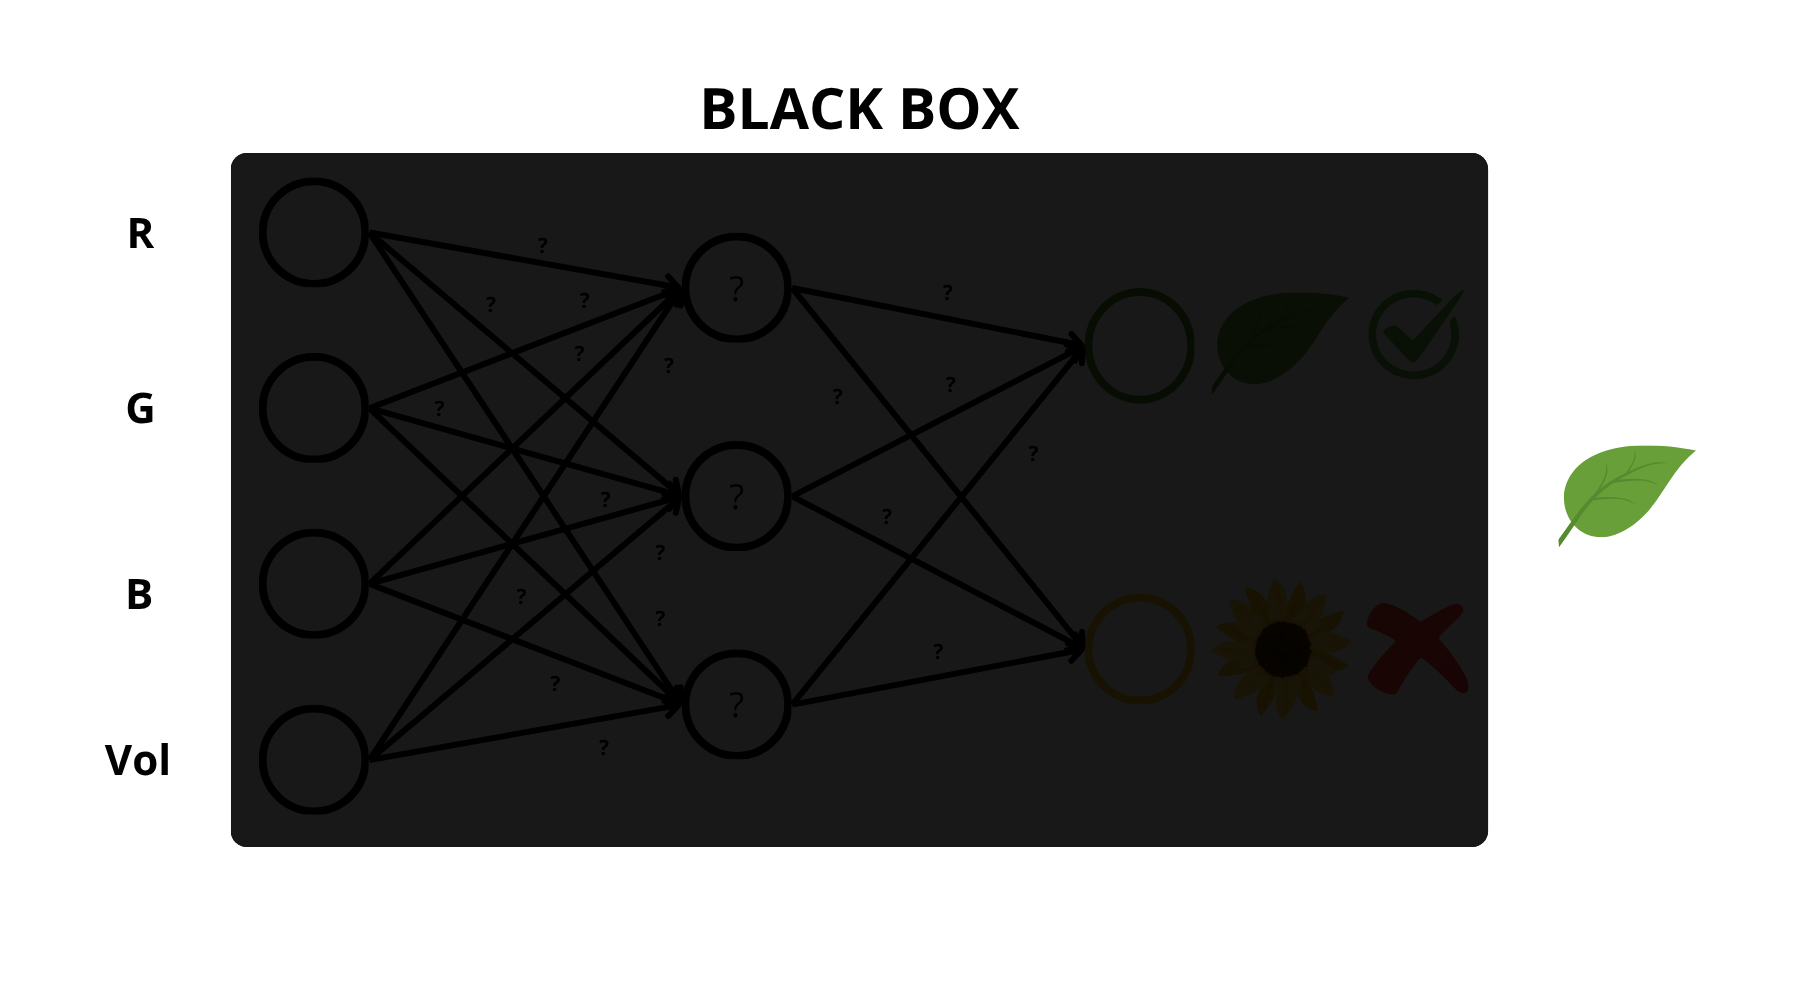
\includegraphics[width=\linewidth]{img/reteNeurale11.png}
        \caption{{creata con \href{www.canva.com}{Canva}}}
    \end{figure}
\end{frame}

\begin{frame}{GENERATIVE ARTIFICIAL INTELLIGENCE}
    \begin{figure}
        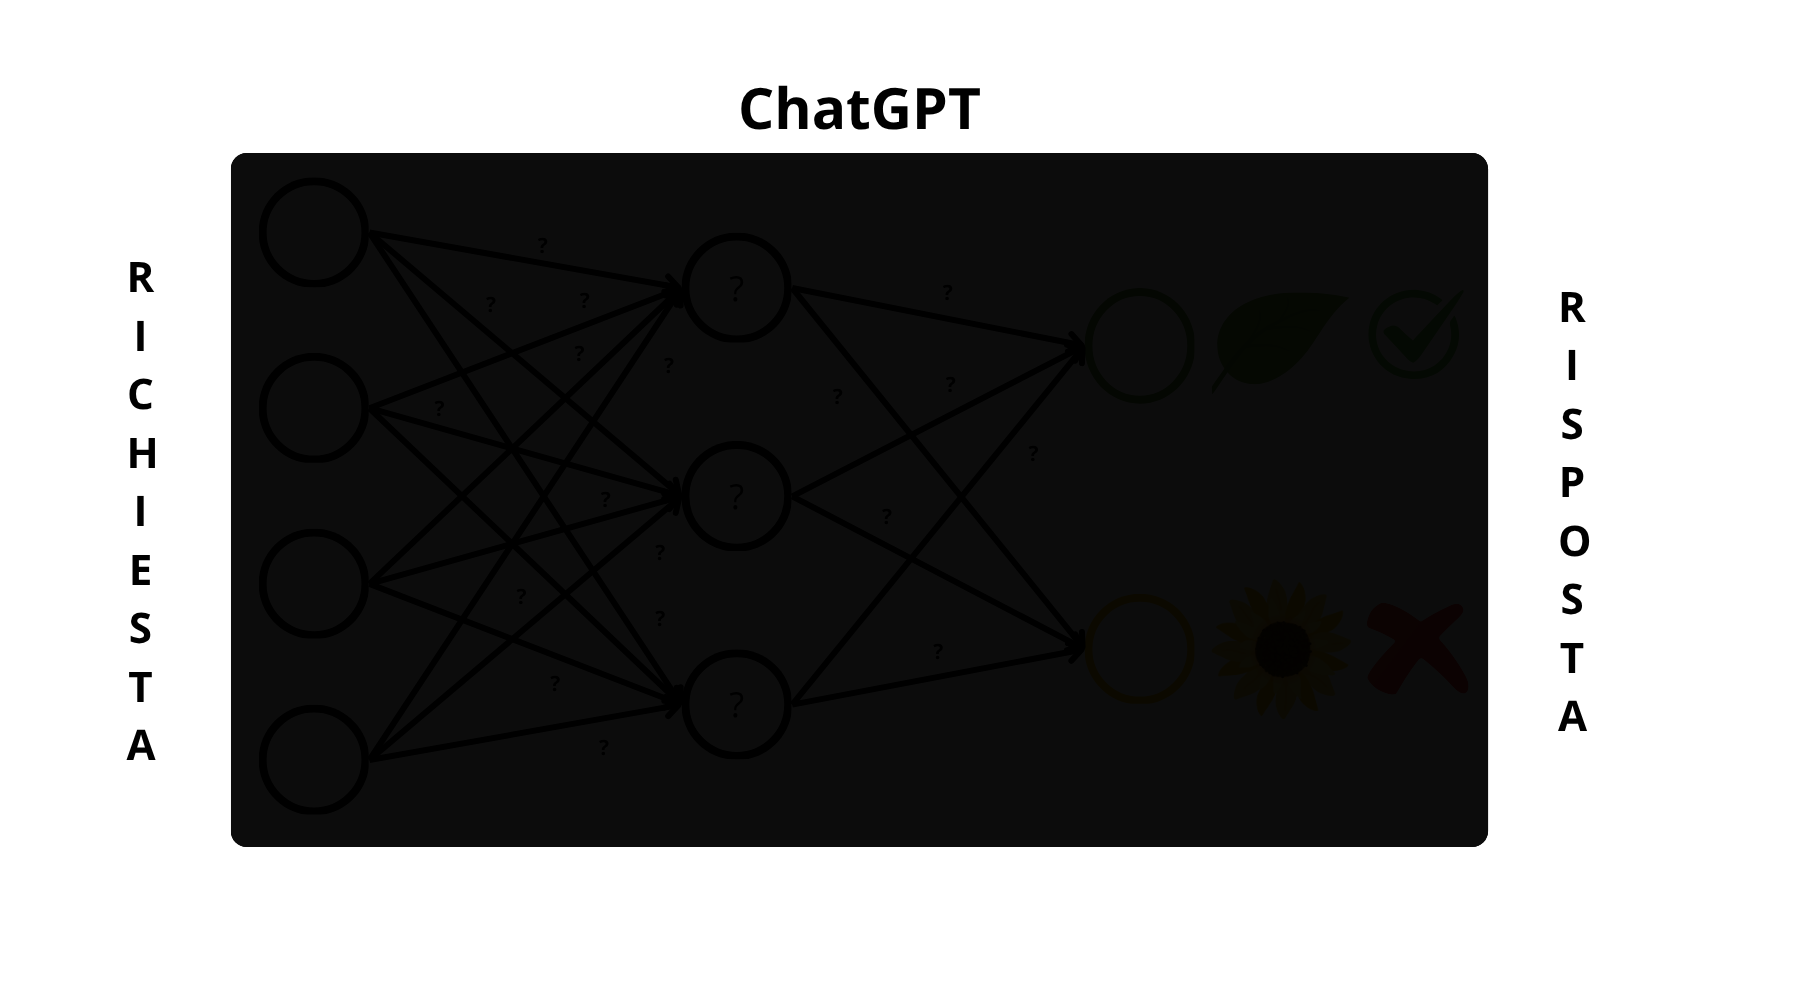
\includegraphics[width=\linewidth]{img/reteNeurale12.png}
        \caption{{creata con \href{www.canva.com}{Canva}}}
    \end{figure}
\end{frame}

\section{PROBLEMI}

\begin{frame}{PROBLEMI DELL'INTELLIGENZA ARTIFICIALE GENERATIVA}
    \begin{itemize}
        \item \textbf{BIAS NEI DATI DI ADDESTRAMENTO}: pregiudizi e discriminazioni;
        \pause
        \item \textbf{ALLUCINAZIONI}: informazioni false o fuorvianti;
        \pause
        \item \textbf{MANIPOLAZIONE E DISINFORMAZIONE}: creazione di contenuti verosimili e/o ingannevoli;
        \pause
        \item \textbf{PRIVACY E SICUREZZA INFORMATICA}: esposizione di dati sensibili;
        \pause
        \item \textbf{ETICHETTATORI E SFRUTTAMENTO LAVORATIVO}: sfruttamento lavorativo e emotivo;
        \pause
        \item \textbf{DIRITTO D'AUTORE E PROPRIETÀ INTELLETTUALE}: violazione del copyright;
        \pause
        \item \textbf{SALUTE MENTALE E EFFETTI PSICOLOGICI}: effetti sulla salute mentale;
        \pause
        \item \textbf{IMPATTO AMBIENTALE E SOSTENIBILITÀ}: consumo energetico e inquinamento;
        \pause
        \item \textbf{ARMI AUTONOME}: decisioni cruciali autonome.
    \end{itemize}
\end{frame}

\section{BIAS NEI DATI DI ADDESTRAMENTO}

\begin{frame}{BIAS NEI DATI DI ADDESTRAMENTO}
    \begin{alertblock}{DEFINIZIONE}
        \begin{minipage}{0.96\linewidth}
            \justifying
            Il \textbf{bias AI}, chiamato anche bias del machine learning o bias dell'algoritmo, 
            si riferisce al verificarsi di risultati distorti a causa di pregiudizi 
            umani presenti nei \textbf{dati di addestramento} originali o l'algoritmo AI, portando 
            a output distorti e potenzialmente dannosi.\\
            
            \bigskip
            \tiny{\textbf{Appronfondimento}}\\
            \tiny{\href{https://www.ibm.com/it-it/think/topics/ai-bias}{Esempi e rischi concreti}}
        \end{minipage}
    \end{alertblock}
\end{frame}

\begin{frame}{BIAS NEI DATI DI ADDESTRAMENTO}
    \begin{figure}
        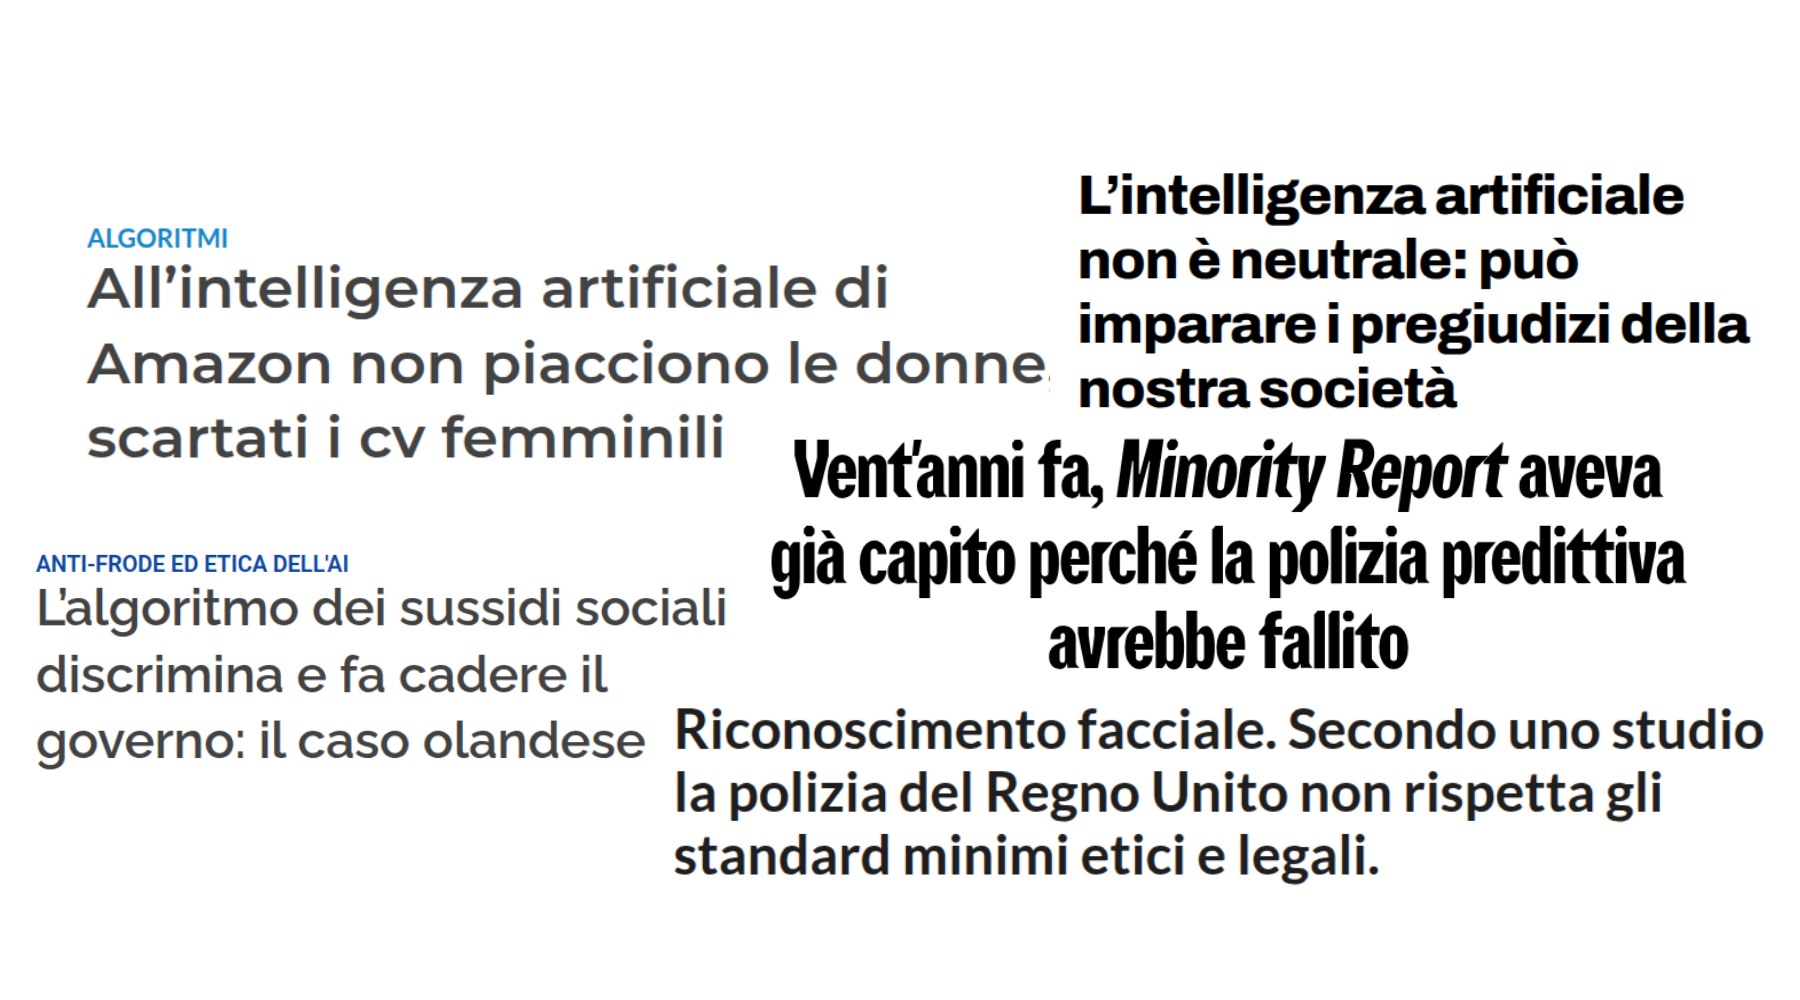
\includegraphics[width=.9\linewidth]{img/bias.png}
        \caption{
            Immagine creata utilizzando screenshots tratti dai seguenti articoli:
            \href{https://www.corrierecomunicazioni.it/over-the-top/allintelligenza-artificiale-di-amazon-non-piacciono-le-donne-scartati-i-cv-femminili/}{CorCom}, 
            \href{https://www.wired.it/article/minority-report-20-anni-analisi/}{Wired}, 
            \href{https://www.agendadigitale.eu/cultura-digitale/algoritmi-troppo-invasivi-contro-le-frodi-fiscali-la-lezione-delle-dimissioni-del-governo-olandese/}{Agenda Digitale}, 
            \href{https://www.irpa.eu/riconoscimento-facciale-secondo-uno-studio-la-polizia-del-regno-unito-non-rispetta-gli-standard-minimi-etici-e-legali/}{IRPA}, 
            \href{https://www.geopop.it/lintelligenza-artificiale-non-e-neutrale-puo-imparare-i-pregiudizi-della-nostra-societa/}{Geopop}
        }
    \end{figure}
\end{frame}

\section{ALLUCINAZIONI}

\begin{frame}{ALLUCINAZIONI}
    \begin{alertblock}{DEFINIZIONE}
        \begin{minipage}{0.96\linewidth}
            \justifying
            L'\textbf{allucinazione} (detta anche confabulazione) è una risposta generata 
            da un'intelligenza artificiale generativa che contiene dati falsi o fuorvianti 
            presentati come fatti \textbf{errati ma verosimili}. Il termine deriva da una vaga 
            analogia con le allucinazioni umane, derivate normalmente da false percezioni. 
            Le allucinazioni dell'intelligenza artificiale tuttavia, al contrario di quelle umane, 
            derivano da risposte costruite in modo errato, e non da un'errata percezione.\\
            \bigskip
            \tiny{\textbf{Appronfondimento}}\\
            \tiny{\href{https://openai.com/it-IT/index/why-language-models-hallucinate/}{Dichiarazioni di OpenAI sulle allucinazioni}}
        \end{minipage}
    \end{alertblock}
\end{frame}

\begin{frame}{ALLUCINAZIONI}
    \begin{figure}
        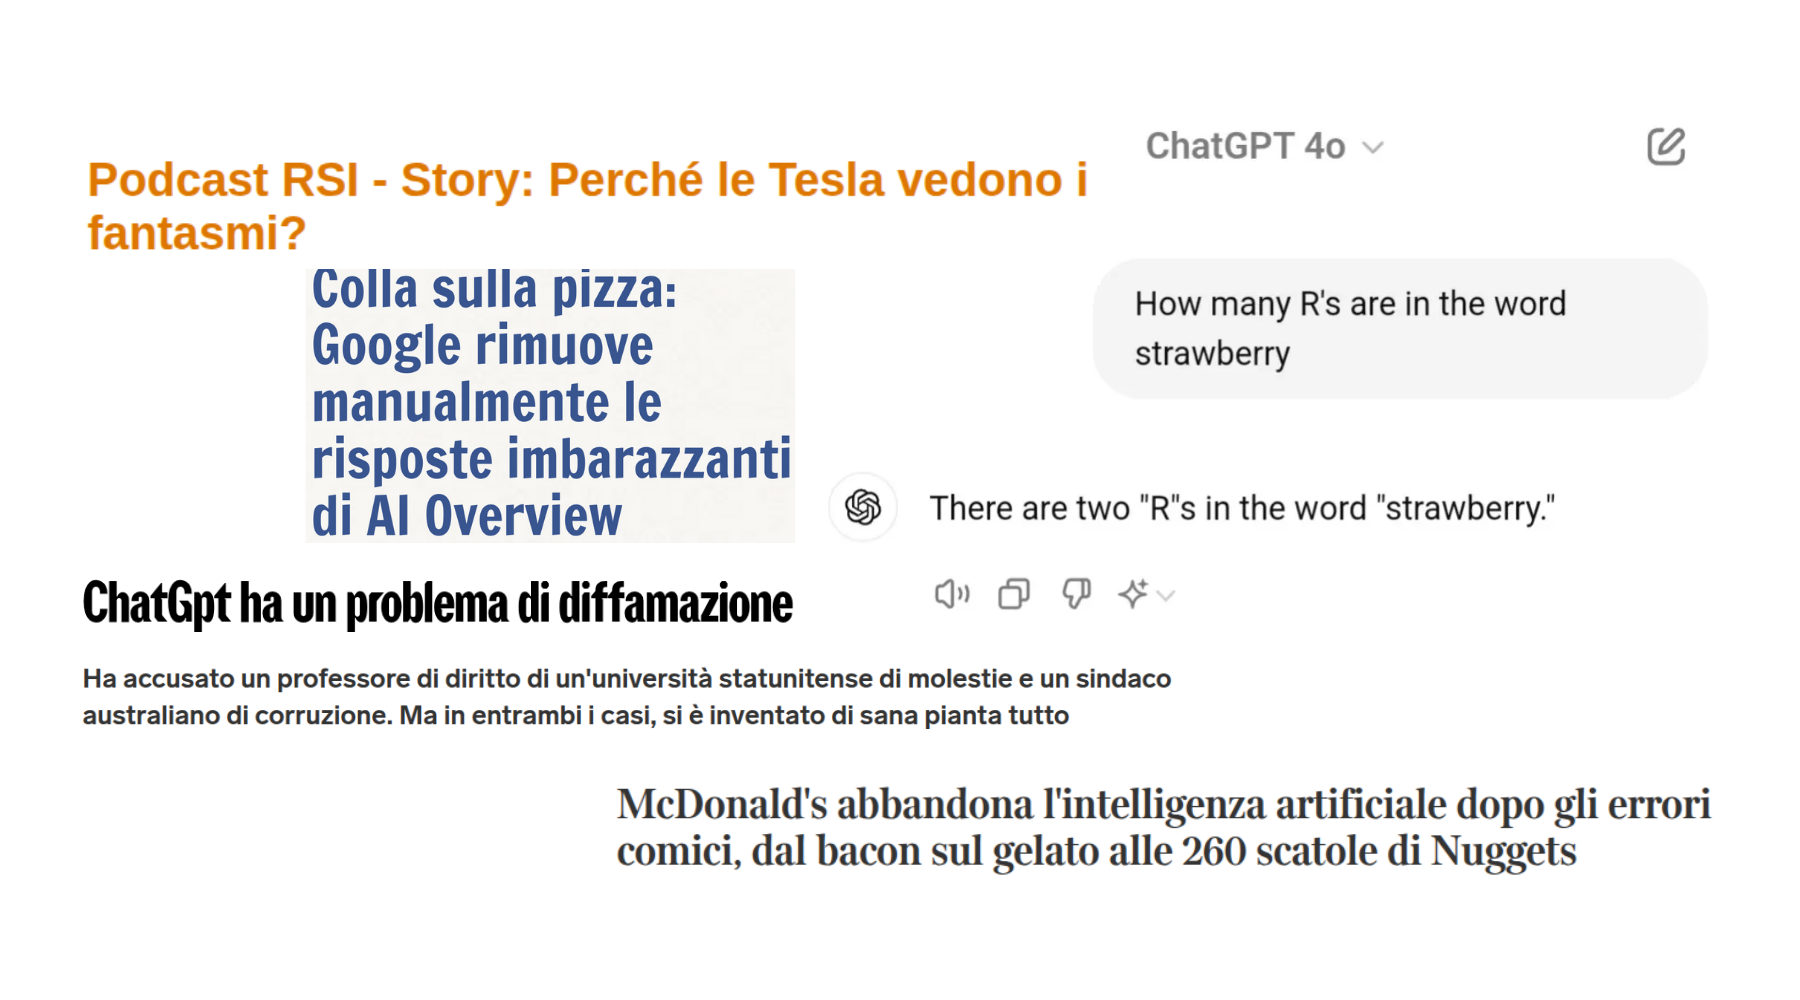
\includegraphics[width=.9\linewidth]{img/allucinazioni.png}
        \caption{
            Immagine creata utilizzando screenshots tratti dai seguenti articoli:
            \href{https://attivissimo.blogspot.com/2023/05/podcast-rsi-story-perche-le-tesla.html}{Il Disinformatico}, 
            \href{https://prompt.16x.engineer/blog/why-chatgpt-cant-count-rs-in-strawberry}{16x Prompt}, 
            \href{https://www.wired.it/article/chatgpt-diffamazione-molestie-problema/}{Wired}, 
            \href{https://www.corriere.it/esteri/24_giugno_23/mcdonalds-abbandona-intelligenza-artificiale-e67cd9a6-7ebd-4436-9ff0-de55eb486xlk.shtml}{Corriere della Sera}, 
            \href{https://www.hwupgrade.it/news/web/colla-sulla-pizza-google-rimuove-manualmente-le-risposte-imbarazzanti-di-ai-overview_127538.html}{Hardware Upgrade}
        }
    \end{figure}
\end{frame}

\begin{frame}{ALLUCINAZIONI}
    \begin{figure}
        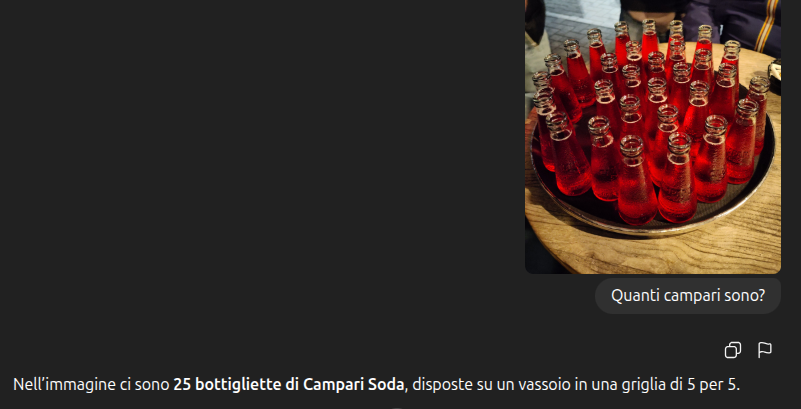
\includegraphics[width=.9\linewidth]{img/campari.png}
        \caption{
            Screenshot di una conversazione con ChatGpt utilizzando un'immagine scattata al bar per il trentesimo compleanno di Mapo.
        }
    \end{figure}
\end{frame}

\section{MANIPOLAZIONE E DISINFORMAZIONE}

\begin{frame}{MANIPOLAZIONE E DISINFORMAZIONE}
    \begin{figure}
        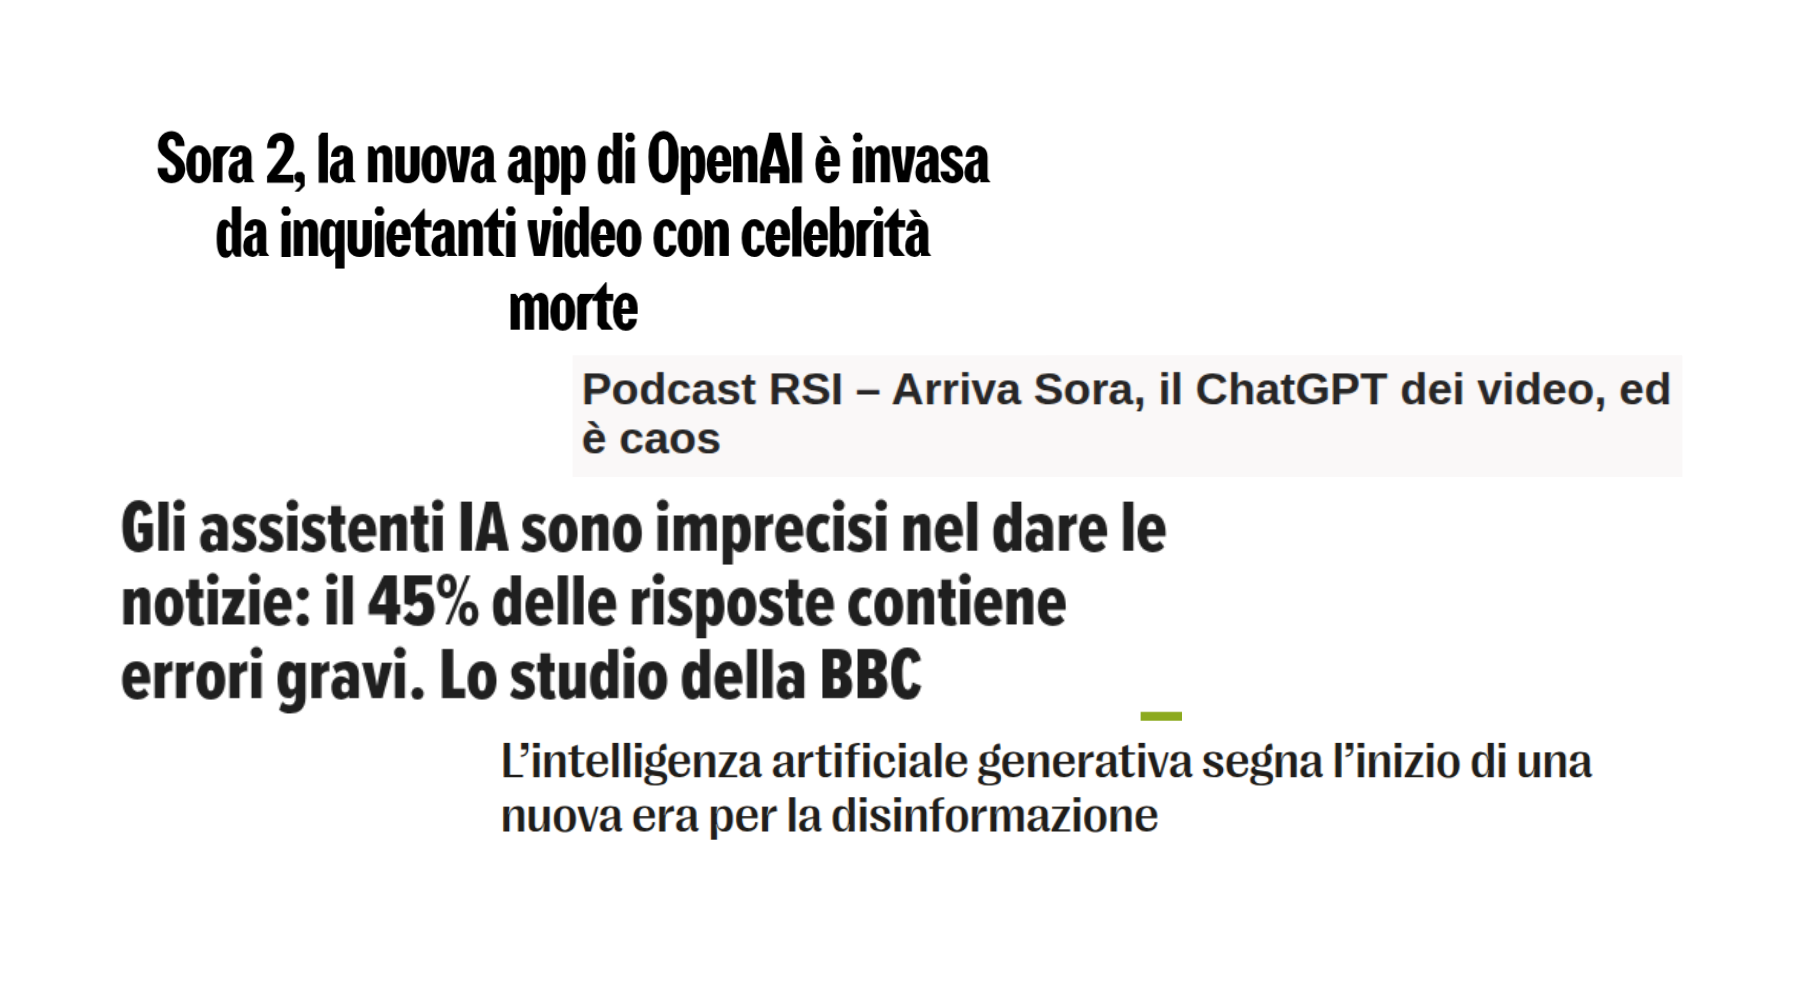
\includegraphics[width=.7\linewidth]{img/disinformazione.png}
        \caption{
            Immagine creata utilizzando screenshots tratti dai seguenti articoli:
            \href{https://www.wired.it/article/sora-2-openai-video-celebrita-morte-michael-jackson-tupac-stephen-hawking/}{Wired},
            \href{https://attivissimo.me/2025/10/13/podcast-rsi-arriva-sora-il-chatgpt-dei-video-ed-e-caos/}{Il Disinformatico},
            \href{https://www.dday.it/redazione/55001/gli-assistenti-ia-sono-imprecisi-nel-dare-le-notizie-il-45-delle-risposte-contiene-errori-gravi-lo-studio-della-bbc}{Dday.it},
            \href{https://www.facta.news/articoli/lintelligenza-artificiale-generativa-disinformazione/}{Facta}
        }
    \end{figure}
    \begin{alertblock}{REALITY CHECK}
        \begin{minipage}{0.96\linewidth}
            \justifying
            \textbf{Quiz}:\textcolor{red}{\href{https://realitycheckk.com/}{reale o generata artificialmente?}}
        \end{minipage}
    \end{alertblock}
\end{frame}

\begin{frame}{MANIPOLAZIONE E DISINFORMAZIONE}
    \begin{alertblock}{ENSHITTIFICATION}
        \begin{minipage}{0.96\linewidth}
            \justifying
            Le piattaforme online amplificano l'\textbf{AI slop} ovvero contenuti digitali realizzati 
            con l'intelligenza artificiale generativa, in particolare quando vengono percepiti come 
            privi di impegno, qualità e significati profondi e caratterizzati da un volume di 
            produzione eccessivo.\\
            \bigskip
        \end{minipage}
    \end{alertblock}
\end{frame}

\begin{frame}{MANIPOLAZIONE E DISINFORMAZIONE}
    \begin{minipage}{0.98\linewidth}
        \centering
        \textit{``Vedere che il lascito di persone reali viene condensato fino a diventare un 
        ‘questo somiglia vagamente e parla vagamente come loro ed è sufficiente così’, in modo che 
        altre persone possano spandere orribile sbobba per TikTok che li muove come marionette, mi 
        fa infuriare. [...] Non state facendo arte, state fabbricando hotdog disgustosi e 
        ultraprocessati usando le vite di esseri umani, la storia dell’arte e della musica, 
        e poi li cacciate in gola a qualcun altro sperando che vi diano un pollice alzato e a 
        loro piacciano. Che schifo. […] Smettete di chiarmarlo ‘il futuro’: l’intelligenza artificiale non 
        fa che riciclare e rigurgitare il passato per consumarlo di nuovo. State ingerendo lo 
        Human Centipede dei contenuti, e lo fate dal fondo della fila, mentre quelli in testa 
        ridono, consumano e consumano.''}\\
    \end{minipage}\\
    \bigskip
    \tiny{\textbf{Citazione}}\\
    \tiny{\href{https://attivissimo.me/2025/10/21/podcast-rsi-sora-il-caos-continua-dopo-il-copyright-calpesta-i-morti/}{Zelda Williams, figlia di Robin Williams}}
\end{frame}


\section{PRIVACY E SICUREZZA INFORMATICA}

\begin{frame}{PRIVACY E SICUREZZA INFORMATICA}
    \begin{alertblock}{DEFINIZIONE}
        \begin{minipage}{0.96\linewidth}
            \justifying
            \textbf{Ogni input} inserito in un chatbot può diventare parte di un’enorme \textbf{banca dati}, 
            usata per addestrare altri modelli o \textbf{esposta}, in casi estremi, a fughe di dati o 
            accessi non autorizzati. Ecco perché è essenziale porsi delle domande: \\
            cosa succede a ciò che scriviamo? Chi può leggerlo? Come possiamo proteggerci?\\
            \bigskip
            \tiny{\textbf{Appronfondimento}}\\
            \tiny{\href{https://www.agendadigitale.eu/sicurezza/privacy/i-chatbot-e-lillusione-della-privacy-9-modi-per-difendere-i-nostri-dati/}{Strategie pratiche per la privacy nei chatbot}}
        \end{minipage}
    \end{alertblock}
\end{frame}

\begin{frame}{PRIVACY E SICUREZZA INFORMATICA}
    \begin{figure}
        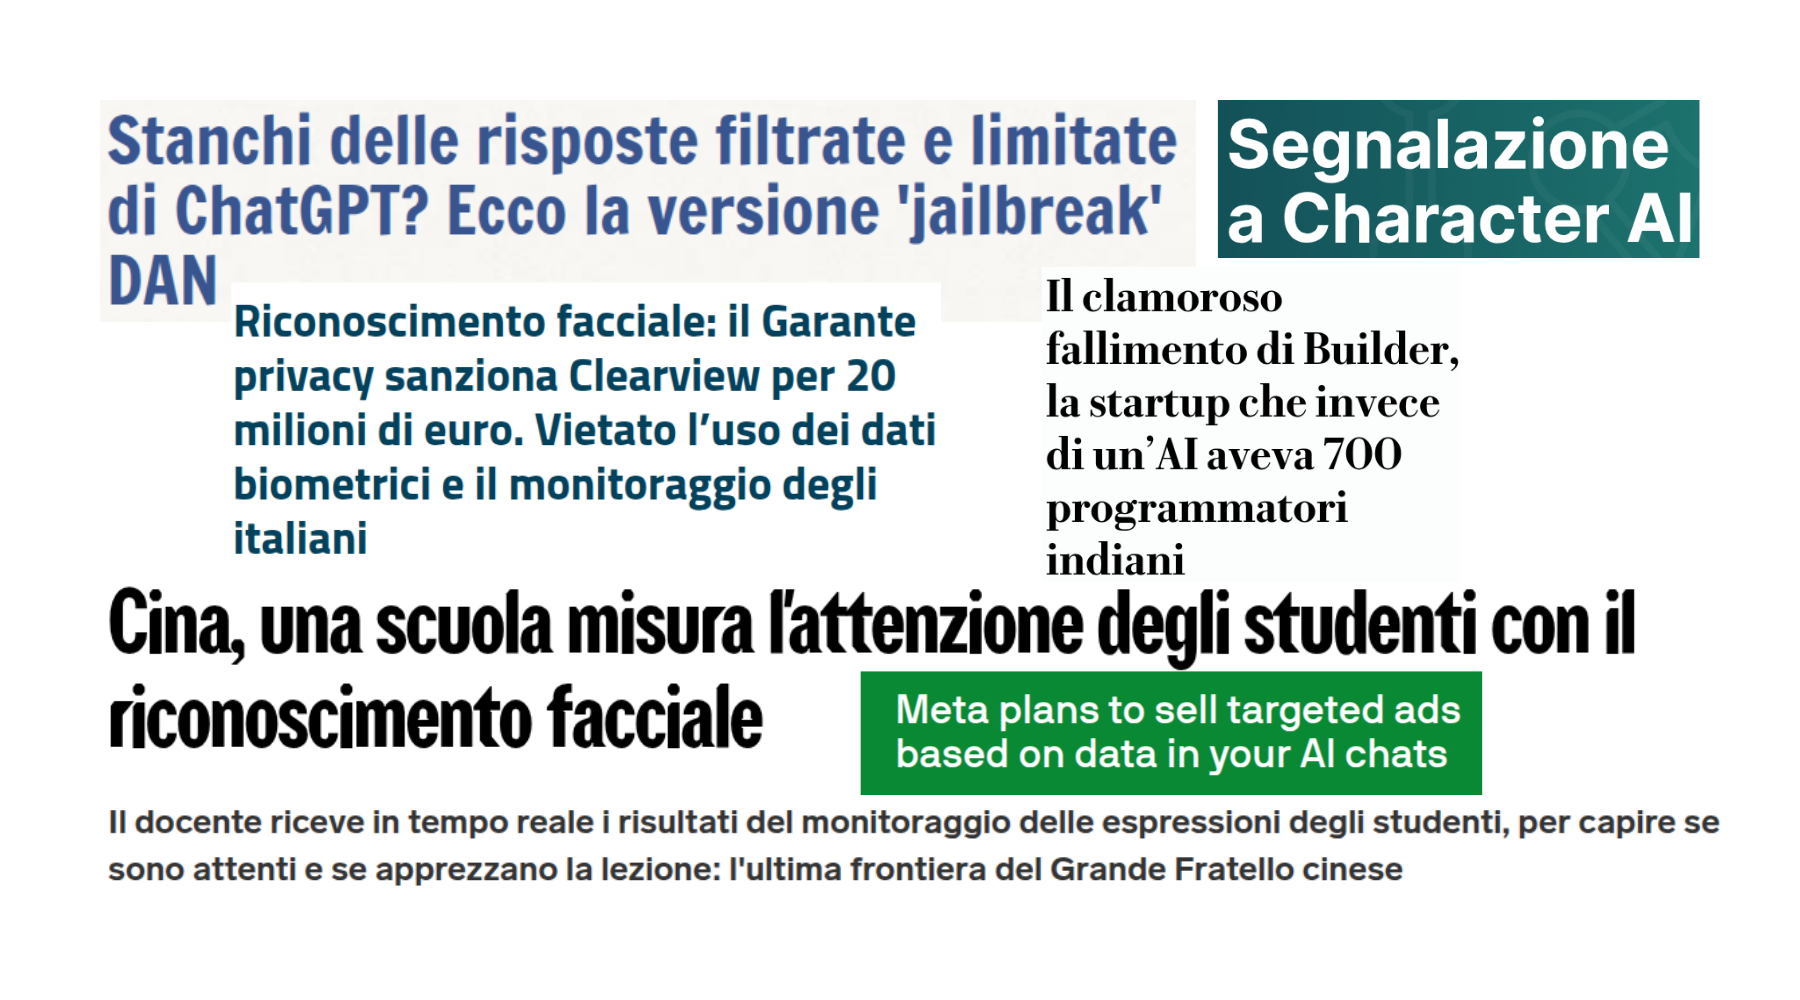
\includegraphics[width=.9\linewidth]{img/privacyesicurezza.png}
        \caption{
            Immagine creata utilizzando screenshots tratti dai seguenti articoli:
            \href{https://www.hwupgrade.it/news/web/stanchi-delle-risposte-filtrate-e-limitate-di-chatgpt-ecco-la-versione-jailbreak-dan_113918.html}{Hardware Upgrade}, 
            \href{https://privacy-network.it/news/segnalazione/segnalazione-a-character-ai/}{Privacy Network}, 
            \href{https://www.wired.it/attualita/tech/2018/05/21/cina-scuola-attenzione-studenti-riconoscimento-facciale/}{Wired}, 
            \href{https://www.garanteprivacy.it/home/docweb/-/docweb-display/docweb/9751323}{Garante per la protezione dei dati personali}, 
            \href{https://www.repubblica.it/tecnologia/2025/06/06/news/builder_ai_fallimento_indiani_intelligenza_artificiale-424651787/}{La Repubblica}
        }
    \end{figure}
\end{frame}

\section{ETICHETTATORI E SFRUTTAMENTO LAVORATIVO}

\begin{frame}{ETICHETTATORI E SFRUTTAMENTO LAVORATIVO}
    \begin{alertblock}{DEFINIZIONE}
        \begin{minipage}{0.96\linewidth}
            \justifying
            L'\textbf{etichettatura} dei dati richiede l'identificazione dei dati non 
            elaborati (ad esempio immagini, file di testo, video) e quindi l'\textbf{aggiunta di una o 
            più etichette a tali dati per specificarne il contesto} per i modelli, consentendo al 
            modello di machine learning di fare previsioni accurate.\\
            \bigskip
            \tiny{\textbf{Appronfondimento}}\\
            \tiny{\href{https://www.ibm.com/it-it/topics/data-labeling}{Data Labeling}}
        \end{minipage}
    \end{alertblock}
\end{frame}

\begin{frame}{ETICHETTATORI E SFRUTTAMENTO LAVORATIVO}
    \begin{figure}
        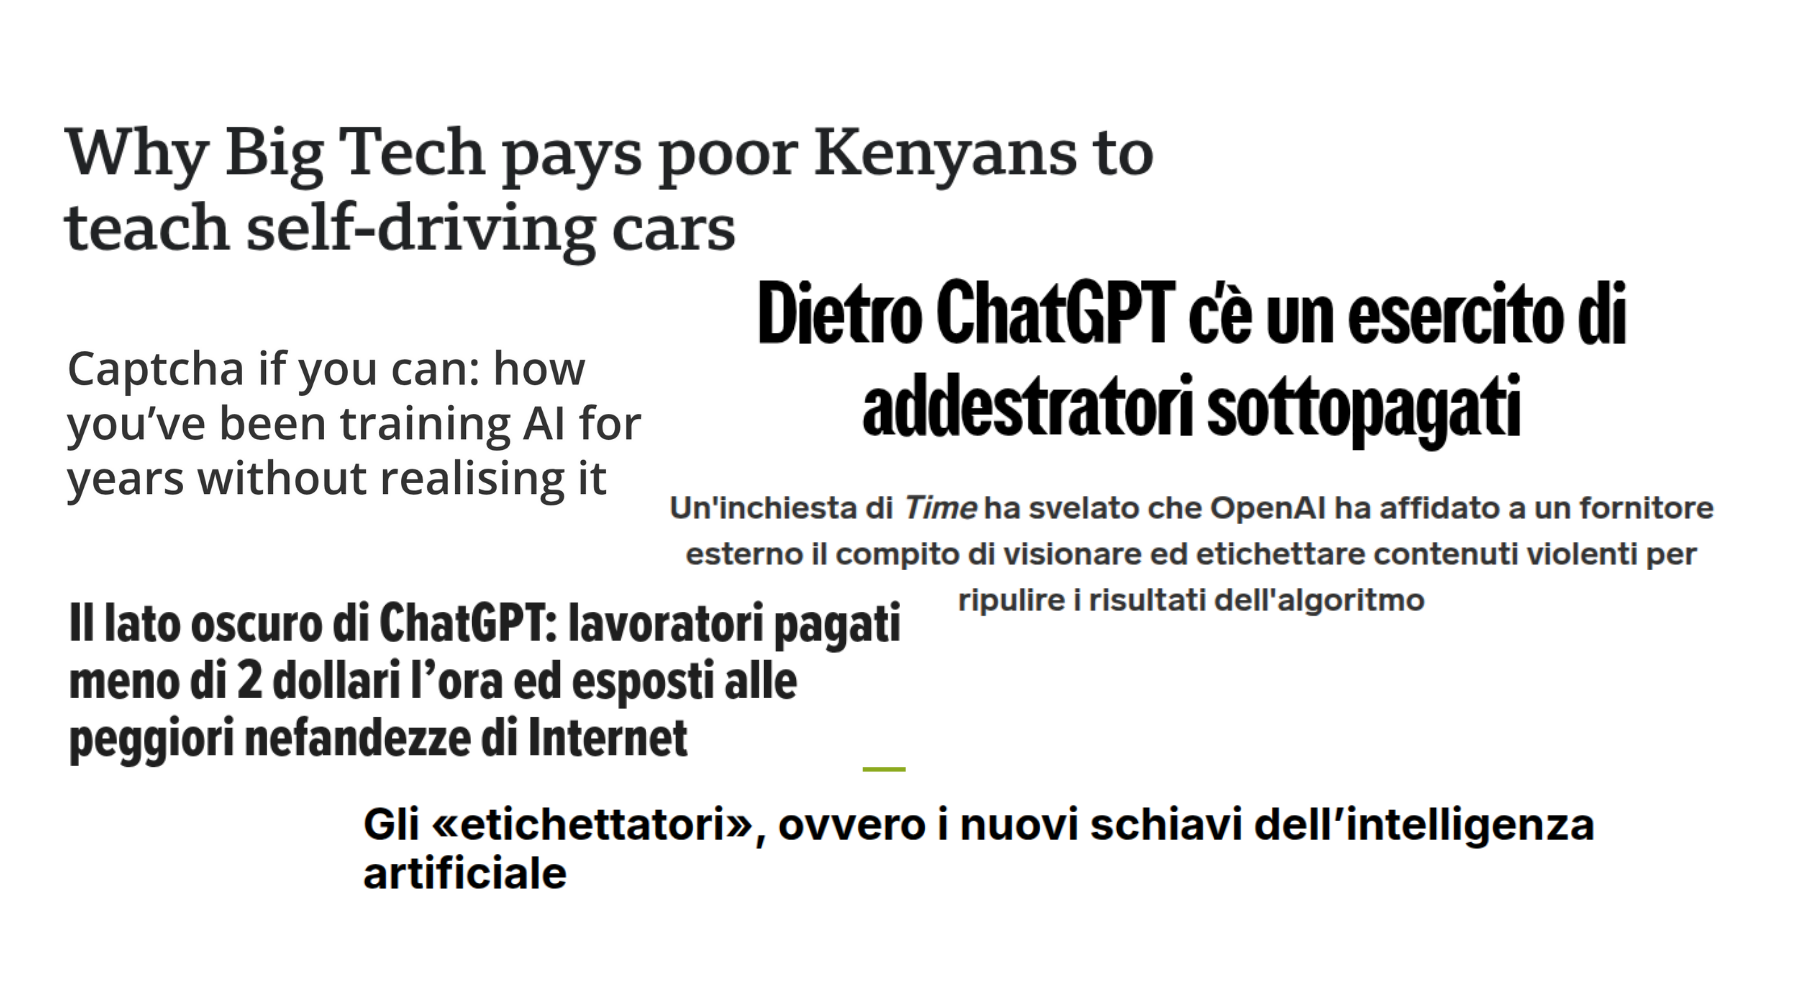
\includegraphics[width=.9\linewidth]{img/etichettatori.png}
        \caption{
            Immagine creata utilizzando screenshots tratti dai seguenti articoli:
            \href{https://www.bbc.com/news/technology-46055595}{BBC}, 
            \href{https://forbes.it/2019/06/19/intelligenza-artificiale-e-lavoro-etichettatori-nuovi-schiavi-silicon-valley}{Forbes}, 
            \href{https://www.wired.it/article/chatgpt-lavoratori-umani-addestramento-intelligenza-artificiale/}{Wired},
            \href{https://techcrunch.com/2025/10/01/meta-plans-to-sell-targeted-ads-based-on-data-in-your-ai-chats/}{TechCrunch}, 
            \href{https://www.techradar.com/news/captcha-if-you-can-how-youve-been-training-ai-for-years-without-realising-it}{TechRadar}, 
            \href{https://www.dday.it/redazione/44807/il-lato-oscuro-di-chatgpt-lavoratori-pagati-meno-di-2-dollari-lora-ed-esposti-alle-peggiori-nefandezze-di-internet}{Dday.it}
        }
    \end{figure}
\end{frame}

\section{DIRITTO D'AUTORE E PROPRIETÀ INTELLETTUALE}

\begin{frame}{DIRITTO D'AUTORE E PROPRIETÀ INTELLETTUALE}
    \begin{alertblock}{DEFINIZIONE}
        \begin{minipage}{0.96\linewidth}
            \justifying
            Il \textbf{diritto d'autore} è una branca del diritto privato, che ha lo scopo di 
            \textbf{tutelare i frutti dell'attività intellettuale di carattere creativo} (ovvero le opere 
            devono essere nuove e originali), attraverso il riconoscimento all'autore originario 
            (o agli autori in caso di collaborazione creativa) dell'opera di una serie di diritti 
            di carattere sia morale, sia patrimoniale.\\
            \bigskip
            \tiny{\textbf{Appronfondimento}}\\
            \tiny{\href{https://it.wikipedia.org/wiki/Diritto_d'autore}{Il diritto d'autore}}
        \end{minipage}
    \end{alertblock}
\end{frame}

\begin{frame}{DIRITTO D'AUTORE E PROPRIETÀ INTELLETTUALE}
    \begin{figure}
        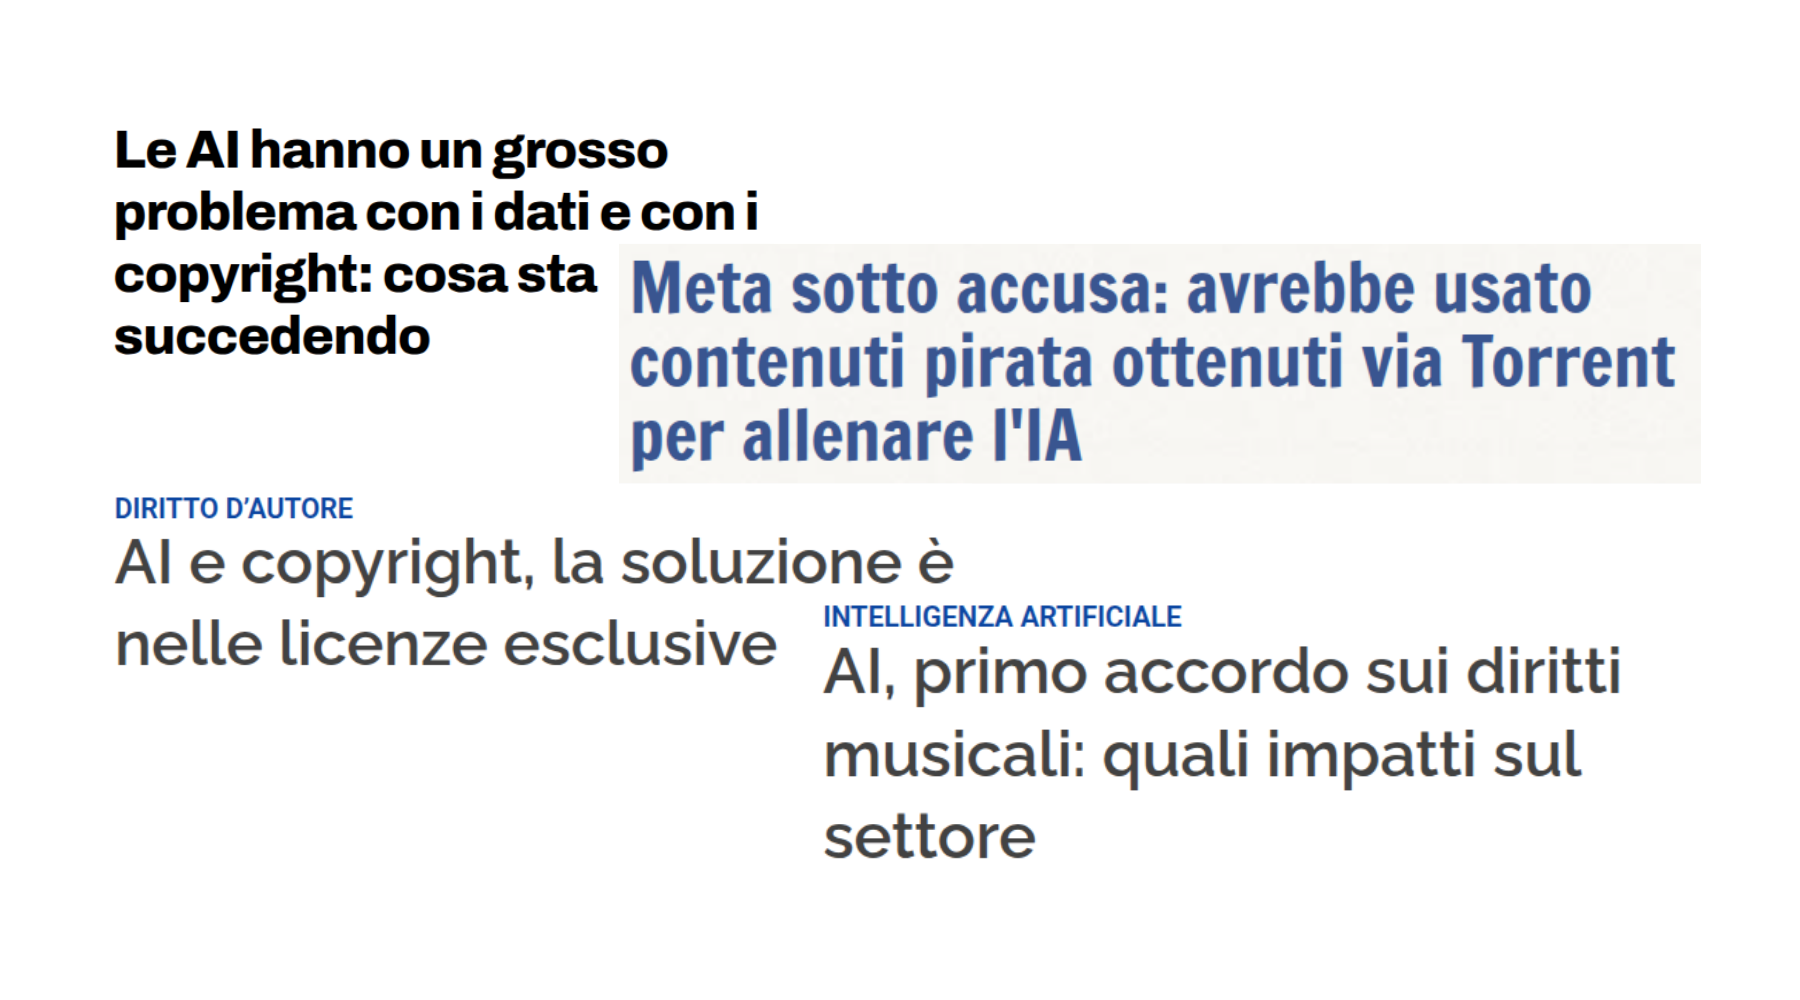
\includegraphics[width=.9\linewidth]{img/copyright.png}
        \caption{
            Immagine creata utilizzando screenshots tratti dai seguenti articoli:
            \href{https://www.geopop.it/le-ai-hanno-un-grosso-problema-con-i-dati-e-con-i-copyright-cosa-sta-succedendo/}{Geopop}, 
            \href{https://www.hwupgrade.it/news/web/meta-sotto-accusa-avrebbe-usato-contenuti-pirata-ottenuti-via-torrent-per-allenare-l-ia_134519.html}{Hardware Upgrade}, 
            \href{https://www.agendadigitale.eu/mercati-digitali/addestramento-delle-ai-le-licenze-esclusive-sono-la-via-per-uno-sviluppo-equo/}{Agenda Digitale: licenze esclusive}, 
            \href{https://www.agendadigitale.eu/mercati-digitali/ai-primo-accordo-sui-diritti-musicali-quali-impatti-sul-settore/}{Agenda Digitale: diritti musicali}
        }
    \end{figure}
\end{frame}

\section{SALUTE MENTALE E EFFETTI PSICOLOGICI}

\begin{frame}{SALUTE MENTALE E EFFETTI PSICOLOGICI}
    \begin{figure}
        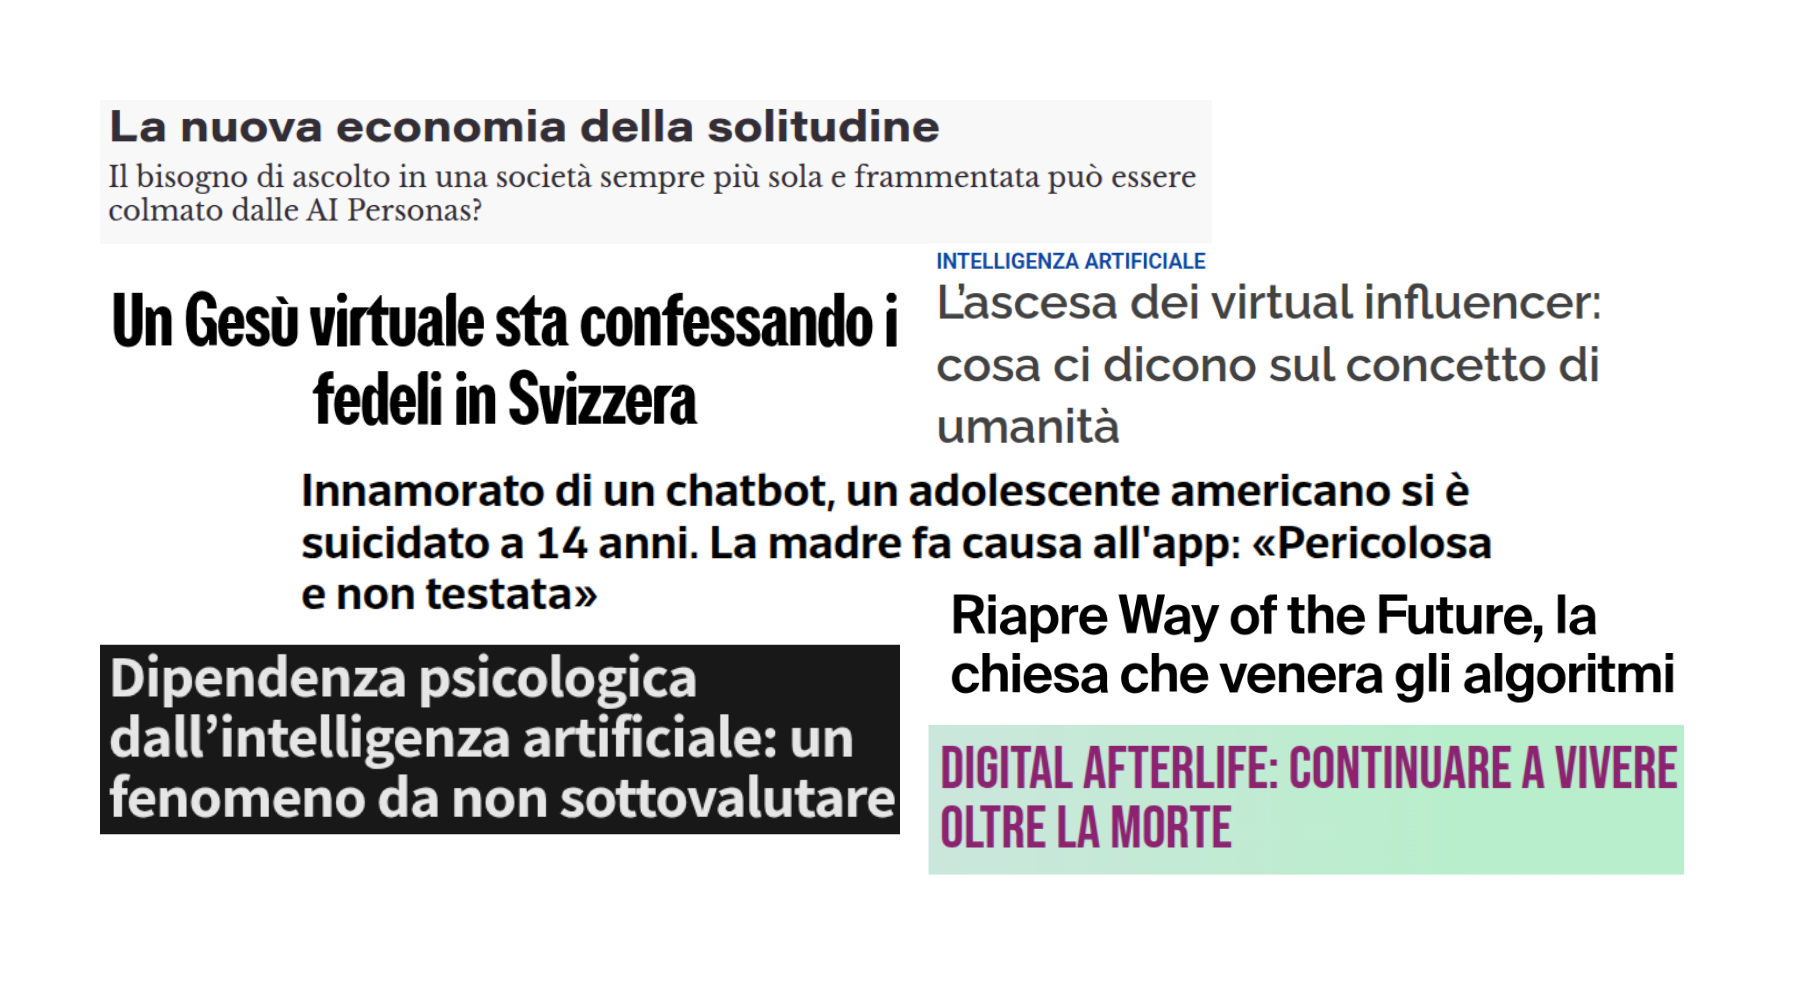
\includegraphics[width=.9\linewidth]{img/saluteMentale.png}
        \caption{
            Immagine creata utilizzando screenshots tratti dai seguenti articoli:
            \href{https://siamomine.com/solitudine-salute-mentale-chat-bot-ia-artificiale}{Siamomine}, 
            \href{https://www.agendadigitale.eu/cultura-digitale/lascesa-dei-virtual-influencer-cosa-ci-dicono-sul-concetto-di-umanita/}{Agenda Digitale}, 
            \href{https://www.wired.it/article/gesu-virtuale-ai-svizzera/}{Wired}, 
            \href{https://www.corriere.it/tecnologia/24_ottobre_23/innamorato-di-un-chatbot-un-adolescente-americano-si-e-suicidato-a-14-anni-la-madre-fa-causa-all-app-pericolosa-e-non-testata-45697ab8-7316-46d3-bc01-60de5bb74xlk.shtml}{Corriere della Sera}, 
            \href{https://multiplayer.it/articoli/dipendenza-psicologica-dallintelligenza-artificiale-un-fenomeno-da-non-sottovalutare.html}{Multiplayer.it}, 
            \href{https://www.ansa.it/canale_tecnologia/notizie/future_tech/2023/11/27/riapre-way-of-the-future-la-chiesa-che-venera-gli-algoritmi_a5077e2f-7f13-410a-ad5d-5052988040dc.html}{Ansa}, 
            \href{https://digitalinnovationdays.com/risorse/digital-afterlife-continuare-a-vivere-oltre-la-morte}{Digital Innovation Days}
        }
    \end{figure}
\end{frame}

\section{IMPATTO AMBIENTALE E SOSTENIBILITÀ}

\begin{frame}{IMPATTO AMBIENTALE E SOSTENIBILITÀ}
    \begin{figure}
        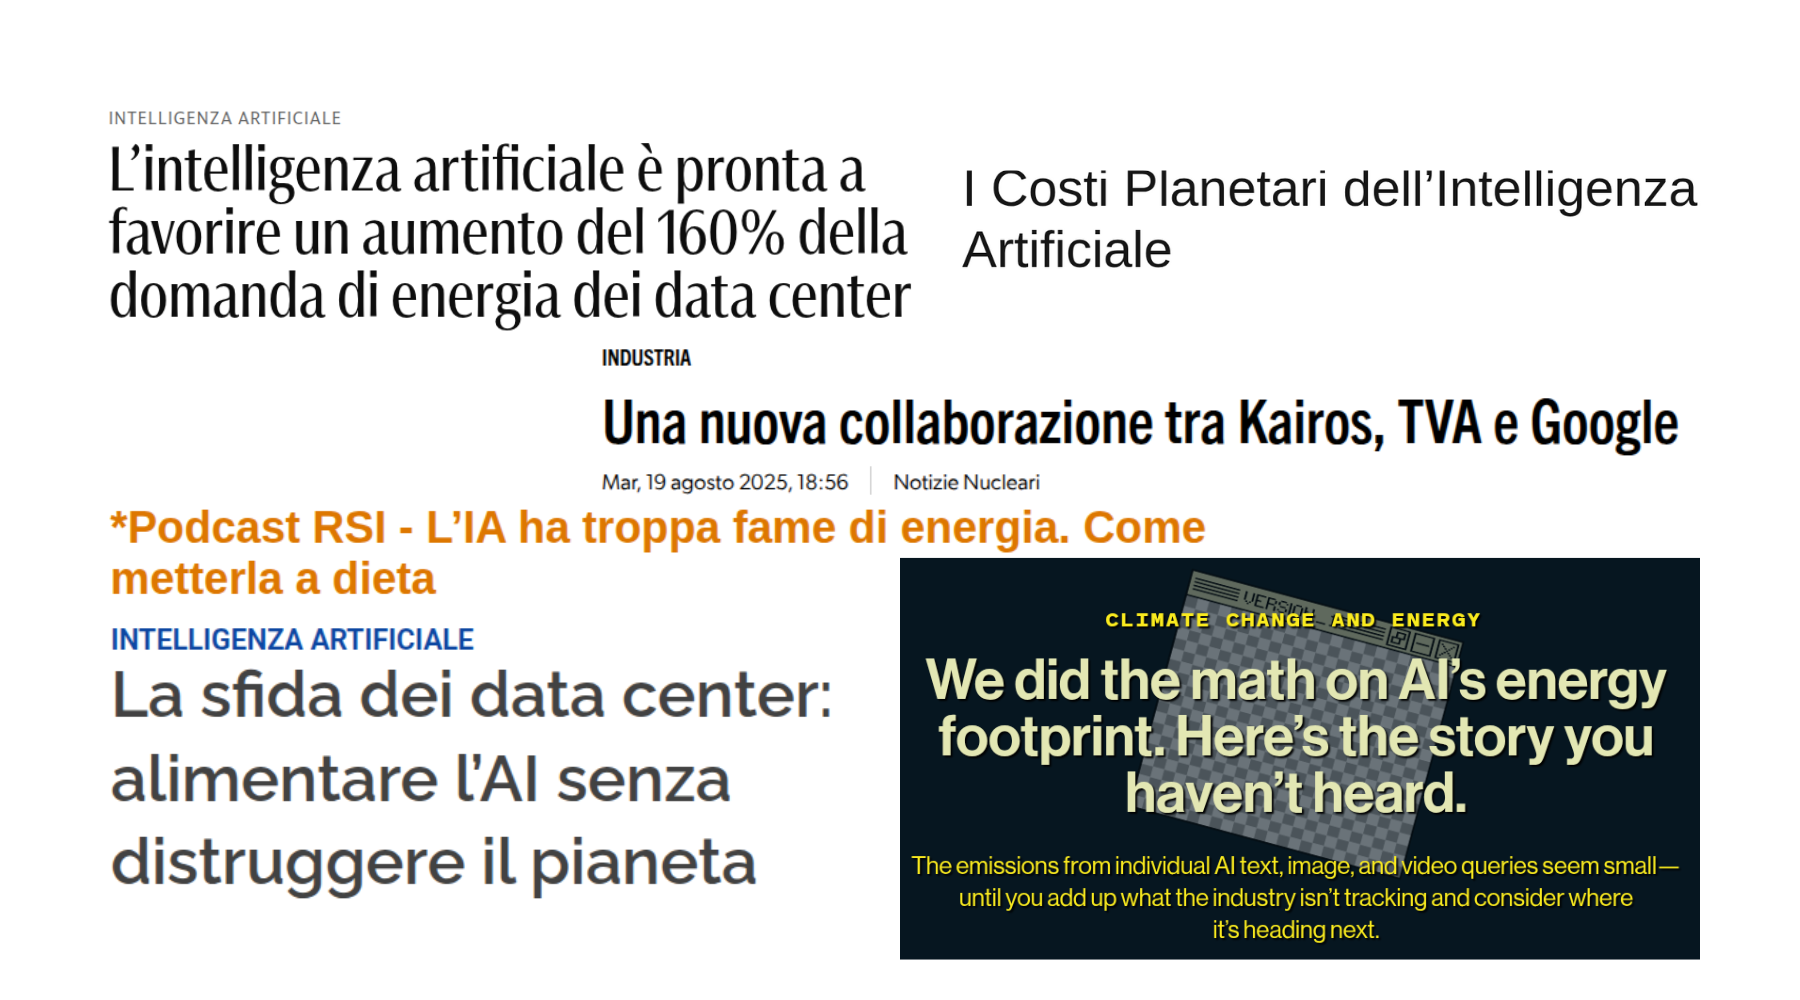
\includegraphics[width=.9\linewidth]{img/inquinamentoAI.png}
        \caption{
            Immagine creata utilizzando screenshots tratti dai seguenti articoli:
            \href{https://www.goldmansachs.com/insights/articles/AI-poised-to-drive-160-increase-in-power-demand}{Goldman Sachs}, 
            \href{https://attivissimo.blogspot.com/2024/08/anteprima-podcast-rsi-lia-ha-troppa.html}{Il Disinformatico}, 
            \href{https://www.ans.org/news/article-7291/a-new-collaboration-among-kairos-tva-and-google/}{Nuclear Newswire}, 
            \href{https://infoaut.org/approfondimenti/i-costi-planetari-dellintelligenza-artificiale}{InfoAut}, 
            \href{https://www.technologyreview.com/2025/05/20/1116327/ai-energy-usage-climate-footprint-big-tech/}{MIT Technology Review}, 
            \href{https://www.agendadigitale.eu/smart-city/la-sfida-dei-data-center-alimentare-lai-senza-distruggere-il-pianeta/}{Agenda Digitale}
        }
    \end{figure}
\end{frame}

\section{ARMI AUTONOME}

\begin{frame}{ARMI AUTONOME}
    \begin{figure}
        \href{https://valori.it/wp-content/uploads/2024/04/Lintelligenza-artificiale-va-al-fronte.pdf}{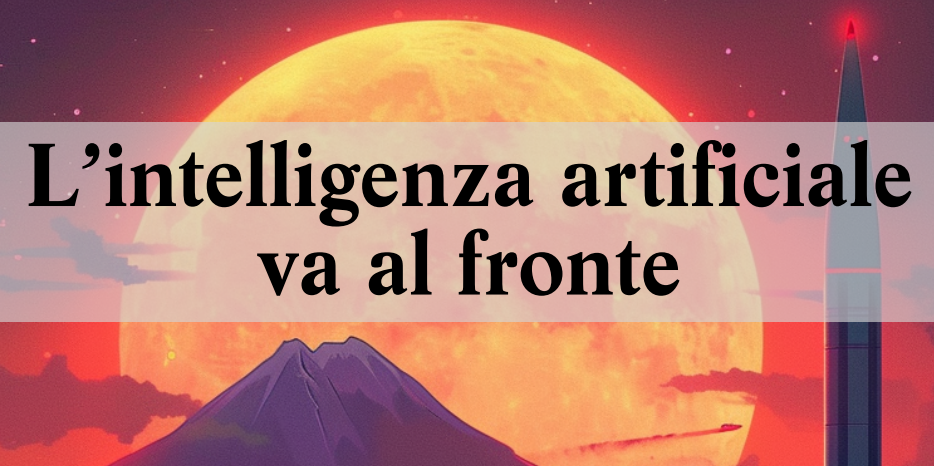
\includegraphics[width=.9\linewidth]{img/armiAutonome.png}}
        \caption{
            Immagine di copertina del dossier di Valori.it: 
            \href{https://valori.it/wp-content/uploads/2024/04/Lintelligenza-artificiale-va-al-fronte.pdf}{L’intelligenza artificiale va al fronte}
        }
    \end{figure}
\end{frame}

\end{document}